 %\documentclass[sigplan,review,anonymous]{acmart}
 %\acmSubmissionID{370} %TODO: Update this after submitting the abstract.
 %\renewcommand\footnotetextcopyrightpermission[1]{}
 % Optional: Remove the ACM reference between the abstract and the main text.
 %\settopmatter{printfolios=true,printacmref=false}
 % Optional: Comment out the CCS concepts and keywords.

%
\documentclass[sigplan,twocolumn,review,anonymous]{acmart}
\acmSubmissionID{111} %TODO: Update this after abstract submission
\renewcommand\footnotetextcopyrightpermission[1]{}
\settopmatter{printfolios=true,printacmref=false}


\usepackage[utf8]{inputenc}
\usepackage{times}
\usepackage{graphicx}
\usepackage{xcolor}
\usepackage{hyperref}
\usepackage{paralist}
\usepackage{listings}
\usepackage[inline]{enumitem}

\usepackage{microtype} % character spacing

\usepackage{booktabs} %added for tables (Andre)
\usepackage{algorithm}
\usepackage[noend]{algpseudocode}
\usepackage{svg}

\usepackage{xparse}
\makeatletter
\NewDocumentCommand{\LeftComment}{s m}{%
	\Statex \IfBooleanF{#1}{\hspace*{\ALG@thistlm}}\(\triangleright\) #2}
\makeatother

\definecolor{dkgreen}{rgb}{0,0.6,0}
\definecolor{gray}{rgb}{0.5,0.5,0.5}
\definecolor{mauve}{rgb}{0.58,0,0.82}
\lstset{language=SQL,
  basicstyle={\scriptsize\ttfamily},
  deletekeywords={key}, %not working
  belowskip=0mm,
  breakatwhitespace=true,
  breaklines=true,
  classoffset=0,
  columns=flexible,
  commentstyle=\color{dkgreen},
  framexleftmargin=0.25em,
  frameshape={}{}{}{},
  %frameshape={}{yy}{}{}, %To remove to vertical lines on left, set `frameshape={}{}{}{}`
  keywordstyle=\color{blue},
  numbers=none, %If you want line numbers, set `numbers=left`
  numberstyle=\tiny\color{gray},
  showstringspaces=false,
  stringstyle=\color{mauve},
  tabsize=3,
  xleftmargin =0em
}

\newcommand{\qcr}[1]{{\fontfamily{qcr}\selectfont #1}}
\newcommand{\code}[1]{\textsf{\small{#1}}}


\usepackage{balance}  % for  \balance command ON LAST PAGE  (only there!)

\usepackage{subcaption}
\graphicspath{{./images/}}

%Makes compact lists a little bit less compact
\setlength{\pltopsep}{0.3em}
\setlength{\plitemsep}{0.1em}

%\newcommand{\grumbler}[2]{{\color{red}{\bf #1:} #2}}
%\renewcommand{\grumbler}[2]{}
%\newcommand{\andre}[1]{\grumbler{andre}{#1}}
%\newcommand{\nuno}[1]{\grumbler{nuno}{#1}}
%\newcommand{\carla}[1]{\grumbler{carla}{#1}}

\newcommand{\outline}[1]{}
%\newcommand{\outline}[1]{\grumbler{outline}{#1}}

\newcommand{\emphvspace}{0.5\baselineskip}
%Single line
\newcommand{\lineemph}[1]{\vspace{\emphvspace}\hspace{2em}\emph{#1}\vspace{\emphvspace}}
%Multi line
\newcommand{\firstblockemph}[1]{\vspace{\emphvspace}\hspace{2em}\emph{#1}}
\newcommand{\middleblockemph}[1]{\hspace{2em}\emph{#1}}
\newcommand{\lastblockemph}[1]{\hspace{2em}\emph{#1}\vspace{\emphvspace}}
\newcommand{\emphfunction}[2]{\emph{#1}($#2$)}

\newtheorem{theorem}{Theorem}

\lstset{columns=fullflexible,
        mathescape=true,
        literate=
               {=}{$\leftarrow{}$}{1}
               {==}{$={}$}{1},
        morekeywords={fun}
        }

\definecolor{red}{RGB}{200,0,0}
\definecolor{green}{RGB}{0,200,0}
\definecolor{blue}{RGB}{0,0,200}
\usepackage{ifthen}
\newboolean{showcomments}
\setboolean{showcomments}{false} %
\ifthenelse{\boolean{showcomments}}
{\newcommand{\nbnote}[3]{
  %
  \fcolorbox{gray}{yellow}{\bfseries\sffamily\scriptsize#1}
  {\color{#2} \sffamily\small$\blacktriangleright$\textit{#3}$\blacktriangleleft$}
%
  %
  }
}
{\newcommand{\nbnote}[3]{}
 \newcommand{\version}{}
}
\newcommand{\andre}[1]{\nbnote{Andre}{blue}{#1}}
\newcommand{\carla}[1]{\nbnote{Carla}{green}{#1}}
\newcommand{\nuno}[1]{\nbnote{Nuno}{red}{#1}}

\begin{document}

%\showthe\columnwidth
%\showthe\textwidth
%\showthe\linewidth

\title{Global Views on Partially Geo-Replicated Data}

%%
%% The "author" command and its associated commands are used to define the authors and their affiliations.
%
%\author{André Rijo, Carla Ferreira, Nuno Preguiça}
%\affiliation{
%\institution{NOVA LINCS, FCT, Universidade NOVA de Lisboa}
%\country{Portugal}
%}

%I used this example provided by VLDB:
%\author{Wang Xiu Ying}
%\author{Zhe Zuo}
%\affiliation{%
%	\institution{East China Normal University}
%	\city{Shanghai}
%	\country{China}
%}
%\email{firstname.lastname@ecnu.edu.cn}

%Maybe the mails should be used separately too as in their example?
%\author{J\"org von \"Arbach}
%\affiliation{%
%	\institution{University of T\"ubingen}
%	\city{T\"ubingen}
%	\country{Germany}
%}
%\email{jaerbach@uni-tuebingen.edu}
%\email{myprivate@email.com}
%\email{second@affiliation.mail}

%Note: from VLDB's guidelines: "list every author in its own author tag. The authors can, as shown in the template sample, share the same affiliations, but every author deserves his/her own author tag! There may not be any Additional Authors section."
%\author{André Rijo}
%\author{Nuno Preguiça}
%\author{Carla Ferreira}
%\affiliation{%
%	\institution{NOVA LINCS, NOVA School of Science and Technology, FCT NOVA}
%	\city{Almada}
%	\country{Portugal}
%}
%\email{a.rijo@campus.fct.unl.pt}
%\email{{nuno.preguica,carla.ferreira}@fct.unl.pt}
%\email{a.rijo@campus.fct.unl.pt, \{nuno.preguica,carla.ferreira\}@fct.unl.pt}

\author{André Rijo}
\affiliation{\institution{NOVA LINCS, NOVA School of Science and Technology of Lisbon}}
\email{a.rijo@campus.fct.unl.pt}
\author{Nuno Preguiça}
\affiliation{\institution{NOVA LINCS, NOVA School of Science and Technology of Lisbon}}
\email{nuno.preguica@fct.unl.pt}
\author{Carla Ferreira}
\affiliation{\institution{NOVA LINCS, NOVA School of Science and Technology of Lisbon}}
\email{carla.ferreira@fct.unl.pt}

\begin{abstract}

%Andre: rewrote Abstract in order to make more clear our novelty and research challenge (mentioned by reviewers 370A, C and D)

Geo-replication is a key technique for providing low latency and high availability in global services.
As the number of data centers increases, so does the replication cost of full replication, 
which makes partial replication attractive.
However, querying over geo-partitioned data is costly and challenging.

This paper presents PotionDB, a novel geo-distributed, partially replicated key-value store with efficient materialized view support.
PotionDB transaction management and replication algorithms provide transactional causal consistency for transactions that access local and remote objects.
Our materialized views enable recurrent queries over geo-partitioned data to be answered locally and efficiently at any replica.
Our evaluation shows that such queries can be completed in sub-millisecond time and achieve high throughput, despite the extra maintenance required to keep views updated.


%Geo-replication is a key technique for providing low latency and high
%availability in global services. As the number of data centers increases, so does the replication cost of full replication, which 
%makes partial replication an attractive approach.

%This paper presents PotionDB, a novel geo-distributed, partially replicated key-value store.  
%PotionDB transaction management and replication algorithms provide transactional causal consistency 
%for transactions that access local and remote objects. 
%To enable the support of recurrent queries over geo-partitioned data, PotionDB provides
%efficient materialized views, that allow these queries to be replied locally at all replicas.
%Our evaluation shows that queries concerning global data can be completed in less than one millisecond 
%while maintaining high throughput, despite the extra operations required to keep views up-to-date. 


%Many existing web services at a global scale have strict latency, availability, and fault tolerance requirements.
%To address these requirements,  services are often deployed in data centers distributed 
%across the globe, with users accessing the closest data center.
%As the number of servers increases, so does the replication cost, which makes partial replication an attractive approach.
%However, some queries may require data not replicated in every server (e.g. in an e-commerce system, the best-selling products across the globe).
%
%In this paper, we present PotionDB, a novel geo-distributed key-value store that provides partial replication.
%We present a replication scheme that allows data to be partially replicated, yet still, answer queries relative to global data efficiently.
%We leverage existing partial and non-uniform replication algorithms to provide materialized views of data that may be split across multiple servers.
%With these views, a client can obtain global information by querying a single server.
%Our evaluation shows that queries concerning global data can be completed in less than one millisecond while maintaining high throughput, despite the extra operations required to keep views up-to-date. 


\end{abstract}

\maketitle

%%% do not modify the following VLDB block %%
%%% VLDB block start %%%
%\pagestyle{\vldbpagestyle}
%\begingroup\small\noindent\raggedright\textbf{PVLDB Reference Format:}\\
%\vldbauthors. \vldbtitle. PVLDB, \vldbvolume(\vldbissue): \vldbpages, \vldbyear.\\
%\href{https://doi.org/\vldbdoi}{doi:\vldbdoi}
%\endgroup
%\begingroup
%\renewcommand\thefootnote{}\footnote{\noindent
%	This work is licensed under the Creative Commons BY-NC-ND 4.0 International License. Visit \url{https://creativecommons.org/licenses/by-nc-nd/4.0/} to view a copy of this license. For any use beyond those covered by this license, obtain permission by emailing \href{mailto:info@vldb.org}{info@vldb.org}. Copyright is held by the owner/author(s). Publication rights licensed to the VLDB Endowment. \\
%	\raggedright Proceedings of the VLDB Endowment, Vol. \vldbvolume, No. \vldbissue\ %
%	ISSN 2150-8097. \\
%	\href{https://doi.org/\vldbdoi}{doi:\vldbdoi} \\
%}\addtocounter{footnote}{-1}\endgroup
%%%% VLDB block end %%%
%
%%%% do not modify the following VLDB block %%
%%%% VLDB block start %%%
%\ifdefempty{\vldbavailabilityurl}{}{
%	\vspace{.3cm}
%	\begingroup\small\noindent\raggedright\textbf{PVLDB Artifact Availability:}\\
%	The source code, data, and/or other artifacts have been made available at \url{\vldbavailabilityurl}.
%	\endgroup
%}
%%%% VLDB block end %%%

\section{Introduction}
\label{sec:introduction}

%	\item Num. DC a aumentar

The increasing reliance on web services in many domains of activity leads to stringent requirements regarding latency, availability,
and fault tolerance~\cite{Schurman2009latency,gomez}.
To address these requirements, cloud platforms have been adding new data centers at different geographic 
locations. By allowing users to contact the closest data center, a global service can
provide low latency to users spread across the globe. 
The increasing number of data centers also contributes
for providing high availability,  as an user can access any
available data center.

% serviços necessitam de data
% Replicar totalmente tem problemas

Global services running at multiple geographic locations rely on a geo-replicated databases~\cite{dynamo, hildred2023caerus, nguyen2023detock}.
%A number of geo-replicated databases have been proposed, providing different consistency semantics.
Databases that provide strong consistency \cite{spanner,cockroachdb,mdcc} give the illusion that 
a single replica exists, requiring coordination among
replicas for executing (update) operations. This leads to high latency and low 
availability in the presence of network partitions.
Databases that provide weak consistency~\cite{eventual,dynamo,cops} allow any replica to process a
client request, leading to lower latency and high availability.These databases expose
temporary state divergence, making it more difficult to program a system. 

In either case, geo-replicated databases usually adopt a full replication model, where each data 
center replicates the full database. 
As both the data managed by these systems and the number of data centers increase,
this approach leads to several problems.
First, storing all data in all data centers imposes a large storage overhead and may be unnecessary, 
as some data is only needed at some locations.
Second, increasing the number of replicas makes replication 
%process 
more complex and costly, 
as each update needs to be propagated to all replicas.

For addressing these problems, partial replication is an attractive approach, with each data center
replicating only a subset of the data.
A number of works have been addressing the challenges of 
partial replication, for example by proposing algorithms to manage partially 
replicated data~\cite{spanner,sipre, practi, hildred2023caerus} and to decide which data is replicated in each replica~\cite{slog, sipre}.

However, querying over a partial, geo-distributed system is challenging, as no single replica has all the necessary data to answer the query. %Andre: trying to make the problem statement more obvious as a followup to reviewers 370A, C and D. TODO: Maybe it would be better to revert this one.
%However, queries requiring a global vision of data are challenging in partial, geo-distributed systems.	
%This paper addresses the problem of querying data in a weakly consistent partially geo-replicated database, 
%focusing on recurrent queries.
For example, consider an e-commerce system with users from multiple geographic locations.
In this case, the data pertaining users of a given location does not need to be replicated in all data centers
(but only in a few for fault tolerance). The same applies to other information, such as data on orders and 
warehouses.
Other data, such as information on products would be replicated in the regions where the product
is available for sale.  
Under this data placement, computing the list of best seller products is challenging, as it requires
accessing data located at multiple data centers.

This paper addresses this problem. %
%This problem can be addressed using different approaches. 
A possible solution is to
%First, it is possible to 
have a \emph{main} data center that replicates all data, and forward queries to such data center.
This makes the \emph{main} data center a central point of failure and a performance bottleneck, as it needs to execute all these queries.
%Second, 
Alternatively, 
it is possible to execute the query by accessing multiple locations, using, for example, 
a distributed processing system for geo-partitioned data~\cite{kloudas2015pixida,jetstream}.
This requires running an additional external service, posing challenges for the consistency of these results and 
queries executed in the database.
The same problems occurs when caching results of these queries~\cite{chronocache}.
%, mostly when adopting weak consistency models (a local update that should
%be reflected in the result of the query may not be returned, as the update might have not been read by the 
%external service that accessed a different replica).

We propose a different approach: to maintain materialized views for recurrent queries.
%, as commonly available in centralized 
%relational databases. 
Although the frequency of recurrent
queries depends on the application, the popularity of application caches (e.g. memcached and Redis)  
and database caches \cite{chronocache} shows that recurrent queries are common in practice.
Implementing such feature efficiently in a partially geo-replicated database requires 
addressing two main challenges. 
First, it is necessary to maintain the materialized views consistent with the remaining data
accessed by the application. 
To achieve this, we designed mechanisms for transaction execution and replication where updates 
to the base data and views are made visible atomically in each replica.

Second, it is necessary to efficiently support materialized views. 
Our key insight is that most updates do not affect the state of views for
common recurrent queries with aggregations or limits (e.g. TPC-H~\cite{tpch} queries).
We have designed an incremental view maintenance mechanism that only propagates the
necessary updates, which builds and extends 
Non-uniform Conflict-free Replicated Data Types (NuCRDTs)~\cite{Cabrita17Nonuniform}.
%, a CRDT~\cite{crdt} model where each replica can maintain a different state as long as the 
%the results of reads is the same in all replicas. 


%Second, it is necessary to efficiently support materialized views. 
%As many recurrent queries include aggregations or limits (e.g. TPC-H~\cite{tpch})
%%all defined queries use aggregations or limits
%it is particularly important to support these features. 
%We have designed an incremental view maintenance mechanism that builds and extends 
%Non-uniform Conflict-free Replicated Data Types (NuCRDTs)~\cite{Cabrita17Nonuniform}, 
%a CRDT~\cite{crdt} model where each replica can maintain a different state as long as the 
%the results of reads is the same in all replicas. 

%crdt} and non-uniform replication~\cite{Cabrita17Nonuniform}.
%While CRDTs allow updates to views to be performed in any replica, the latter minimizes
%the updates propagated to other replicas to only those that might influence the final result.


%limits, used for example to support \emph{topK} 
%queries.
%To achieve this, we build on the concept of non-uniform replication \cite{Cabrita17Nonuniform}, in which the state
%of different replicas may be different, given that the observable state is (eventually) the same.
%This allows each replica to propagate only the updates that might be relevant to the observable 
%state. Providing support for views required us to extend non-uniform replication from simple data 
%types to more complex structures that could support a view with multiple columns.

We present the design and implementation of PotionDB, a geo-replicated memory key-value store with support  
for partial replication and materialized views. 
PotionDB provides weak consistency, for improved latency and availability,  with transactional 
causal consistency~\cite{cure}, for improved consistency.
Views are kept up-to-date with the base data, allowing replicas to locally return a consistent result to 
recurrent queries over geo-partitioned data.
%Our views enable replicas to locally and efficiently answer recurring queries over geo-partitioned data. %Andre: added this to make more obvious our contribution, as a followup to reviewers 370A, C and D. 
To our knowledge, our work is the first to maintain materialized views in such setting.  

PotionDB was evaluated with \mbox{TPC-H} queries~\cite{tpch} and micro-benchmarks.
The results show that PotionDB provides much better performance to answer recurrent queries
than alternatives.
% approaches.  
Performance scales almost linearly with the number of replicas. % in the system.
Further, the overhead of maintaining materialized views is low, increasing slightly with
\mbox{the ratio of updates.}

% for maintaining materialized views impose 
%low overhead when executing asynchronously replicating transactions, particularly
%for views with limits. 
%\nuno{deviamos ter uns micro-benchmarks que comparassem o overhead com limites e sem limites}
%%Additionally, the results show that executing queries by relying on the materialized views is much more 
%%efficient than using alternative mechanisms.  
%Moreover, our algorithms for maintaining materialized views in a decentralized way perform better 
%than alternative approaches where the view is computed in a single data center, 
%while also keeping consistency between the base and view data in every replica.



In this paper we make the following contributions:
%\begin{enumerate*}[(label=\roman*)]
\begin{itemize}[noitemsep,topsep=0pt,parsep=0pt,partopsep=0pt,leftmargin=*]
	\item 
	%design of a 
	the design of a partially geo-replicated key-value store with 
	views over geo-partitioned data (Section~\ref{sec:transactions}); 
	\item replication algorithms that efficiently maintain consistent materialized views over 
	partially replicated data (Section~\ref{sec:views_for_apps});
%	\item a language inspired in SQL for view specification in key-value stores, with view maintenance code automatically inferred from the specification;
	 \item implementation and evaluation of the proposed approach with TPC-H and micro-benchmarks
	 (Section~\ref{sec:evaluation}).
\end{itemize}

%The remainder of the paper is organized as follows.
%Section~\ref{sec:overview} presents the system model, as well as PotionDB's architecture, consistency guarantees and API. %System model? Or Data Model?
%Section~\ref{sec:transactions} describes PotionDB's transactional and replication protocols.
%Section~\ref{sec:views_for_apps} discusses details on how PotionDB generates views and their automatic updating, as well as how we adapted TPC-H to PotionDB.
%%Section~\ref{sec:views_for_apps} discusses how we adapted TPC-H to PotionDB, exemplifies how views can be specified given a query and discusses some details on how PotionDB generates views and their automatic updating.
%In Section~\ref{sec:evaluation} we experimentally evaluate PotionDB using TPC-H and micro-benchmarks, while Section~\ref{sec:related_work} presents related work and Section~\ref{sec:conclusion} concludes.
%\andre{On the description of Section \ref{sec:views_for_apps}, maybe change "their automatic updating" to "keeps them automatically up-to-date"?}


%\outline{topicos
%
%\begin{itemize}
%	\item Num. DC a aumentar
%	\item Replicar totalmente tem problemas
%	\item Replicação parcial
%	\item Queries sobre dados replicados parcialmente
%	\begin{itemize}
%		\item Standard solution?
%	\end{itemize}
%	\item Views materializadas replicadas totalmente
%	\item Contribuições
%\end{itemize}
%}

\section{System Overview}
\label{sec:overview}

%This section overviews PotionDB, focusing on support for recurrent queries.
%, and in particular for
%complex recurrent queries, such as those present in TPC-H~\cite{tpch}. 

PotionDB is a distributed database designed for supporting global services deployed at multiple data centers. 
In these settings, (some) data items are only needed at some geographic locations. 
As a running example, we consider a large e-commerce site with online stores for different countries 
and clients spread across the world. 
The service includes data for products, with some products available 
only at some locations. The service maintains information about customers and their purchases, 
with clients being associated with one online store.

In this context, fully replicating the whole dataset might become too expensive.
Additionally, as most data is tied to some geographic location, the majority of accesses
occurs on that location. 
PotionDB adopts partial geo-replication, with data items replicated only at some locations.
This allows PotionDB to reduce replication cost when
compared to full replication, saving on both storage, processing, and networking costs.

While some application operations access data objects directly (e.g. user, product, or purchase objects),
other operations require data that results from an aggregation (e.g.  top
selling products worldwide)
%and users that bought some product).  
For supporting the latter, %operations,
PotionDB provides materialized views that are the result of an aggregation 
over geo-partitioned data and provides algorithms to efficiently maintain these views consistent.

Other global services, such as multi-user online games and
social news aggregation, share similar features - having a large database with
data accessed mostly in a single location and operations accessing the result
of a global aggregation.

%The key features of this example - global service with a large database with
%data accessed mostly in a single location and operations accessing the result
%of a global aggregation - are common to other global services, such as multi-user online games, and
%social news aggregation.


%What do I want to define?
%Define formally objects and views.
%Define how objects are identified (key, bucket, type) and the idea of "objectID" (the triple). On the type, can define it generically (set, map, etc. Later can say those map to CRDT types)
%Define the API to process objects. Be short on the common parts of the API. Mention partial reads but in a generic form (give the example of set). Do not mention details on their workings - this will be somewhere else.
%Define the API to define views. I will need to think of this carefully, as we do not really have an API for this.
%Maybe can be something like saying views are just like normal objects... the detail is on how to keep them updated, and leave that for another section.

\subsection{Data model}
\label{subsec:datamodel}

PotionDB is a distributed key-value database.
We identify two types of values: base objects, $\mathit{Objs}$, and derived objects, $\mathit{Views}$.
The set of objects of a database is defined as $\mathit{DB} = \mathit{Objs} \cup \mathit{Views}$.
Informally, an object, $o$, is any value that is either a base object, $b$, or view, $v$.
We distinguish between base objects and views whenever necessary for clarity.

The value of a view is a function over the values of other object(s), i.e., 
$\forall\, v \in \mathit{Views} : v = \mathit{fun}_v(D_v)$, 
with $D_v$  the set of base and derived objects used to compute $v$.
We assume the computation is non-recursive, i.e., the value of a view is never based on its own value or, formally, 
$\forall\, v \in \mathit{Views} : v \notin D_v$.

Objects are uniquely identified by a tuple $\mathit{id} = \mathit{(key, bucket}$, $\mathit{type)}$.
%For presentation purposes, we assume this tuple is a property of the object and we define $\mathit{id} = \mathit{(key, bucket, type)}$.
%When needed, we represent these properties for an object $o$ as
%$o^{\mathit{id}}$, $o^{\mathit{key}}$, $o^{\mathit{bucket}}$, $o^{\mathit{type}}$.
Objects are stored in $\mathit{buckets}$, which are the unit of replication in PotionDB. 
Buckets are further logically grouped in containers. %, as further detailed in Section \ref{subsec:buckets}. 
An object has a $\mathit{key}$ inside the bucket.

PotionDB supports objects of different data types, including registers, counters, averages, sets, maps
and top-K objects~\cite{Cabrita17Nonuniform}.
Both base object and views are implemented as CRDTs~\cite{crdt}, guaranteeing that object replicas converge to a single state
in the presence of concurrent updates.

\subsection{Interface}
\label{subsec:interface}

%<<<<<<< HEAD
%\begin{table}[]
%	\setlength\tabcolsep{4pt}
%	\begin{tabular}{ll} 
%		\toprule
%		\hspace*{-0.35em}get(txId, id) $\rightarrow$ value                  & begin(clk) $\rightarrow$ txId            \\
%		\hspace*{-0.35em}read(txId, id, op) $\rightarrow$ value             & commit(txId) $\rightarrow$ clk           \\
%		\hspace*{-0.35em}update(txId, id, op) $\rightarrow$ ok           & rollback(txId) $\rightarrow$ ok                           \\
%		& \\
%		\hspace*{-0.35em}readTx(clk, read(s)) $\rightarrow$ clk, value(s) & updateTx(clk, update(s)) $\rightarrow$ clk \\
%=======
\begin{smaller}
\begin{table}[t]
\center
	\begin{tabular}{ll} 
		\toprule
		 \code{begin(clk) $\rightarrow$ txId}                    & \code{get(txId, id) $\rightarrow$ value}            \\
		 \code{commit(txId) $\rightarrow$ clk}            & \code{read(txId, id, op) $\rightarrow$ value}          \\
		  \code{rollback(txId) $\rightarrow$ ok}        & \code{upsert(txId, id, op) $\rightarrow$ ok}                        \\[4pt]
		\multicolumn{2}{l}{\code{oneShotTx(clk, (id, op)$^+$) $\rightarrow$ clk, value$^+$}} \\
	%	\multicolumn{2}{l}{\code{updateTx(clk, (id, op)$^+$) $\rightarrow$ clk}} \\
		%\multicolumn{2}{l}{\code{readTx(clk, read$^+$) $\rightarrow$ clk, value$^+$}} \\
		%\multicolumn{2}{l}{\code{updateTx(clk, update$^+$) $\rightarrow$ clk}} \\
		\bottomrule
	\end{tabular}
	%\vspace{0.8em}
	\caption{PotionDB's data manipulation API.}
	\label{table:PotionDB_API}
	\vspace{-20pt}
\end{table}
\end{smaller}

PotionDB offers a transactional key-value interface, as summarized in Table \ref{table:PotionDB_API}.
An application issues interactive transactions, by executing \code{begin(clk)},
where \code{clk} is used to enforce causality between consecutive transactions.
A transaction proceeds with a sequence of operations: 
\begin{inparaenum}[(i)] 
\item \code{get(txId, id)}, which returns the full state of the object;
\item \code{read(txId, id,op)}, which returns the result of read-only operation \code{op} executed in the object; and
\item \code{upsert(txId, id,op)}, which updates object \code{id} by executing operation \code{op}, or creates the object if it does not exist.
%; 
%\item an object is deleted by issuing the \code{delete}  operation.
\end{inparaenum}
Operations defined in each object are type-specific - e.g. a set has a \code{contains(e)} operation to check
if value \code{e} belongs to the set, and an \code{add(e)} and \code{remove(e)} to add or remove \code{e} from the set.
A transaction ends with a \code{commit(txId)} for committing the transaction %, making updates durable,  
or \code{rollback(txId)} to abort the transaction.

%PotionDB also allows an application to issue an one-shot~\cite{eiger} read-only or write-only transaction,
PotionDB also supports one-shot transactions, \code{oneShotTx(clk, (id, op)$^+$)}, that include a sequence of read or
write operations.
%~\cite{??????} 
%read-only or write-only transaction,
%by executing, respectively, \code{readTx(clk, (id, op)$^+$)} or \code{updateTx(clk, (id, op)$^+$)}.
%for aborting 

PotionDB's data definition API includes operations to create and delete buckets, and 
to create views. Even if buckets have no associated
data type,
% i.e., any object type can be stored in any bucket, 
we expect that applications 
store objects of the same type in each bucket.  A document/table row can be stored 
as a map CRDT, with each element of the map having its own type. 


\begin{figure}[t]
\small{
\begin{lstlisting}[language=SQL]
CREATE VIEW (MonthlyTopSales, views) WITH 
YEAR==ANY (SELECT DISTINCT SaleDate.Year FROM sales), 
MONTH==ANY (SELECT DISTINCT SaleDate.Month FROM sales) AS
SELECT ProdName, SaleDate.Month, SaleDate.Year, SUM(Price - Cost) AS SumProfit, COUNT(*) AS NumSales
FROM Sales
WHERE SaleDate.Month == [MONTH] AND SaleDate.Year == [YEAR]
GROUP BY ProdName
ORDER BY SumProfit DESC, NumSales DESC
LIMIT 10
\end{lstlisting}}
	\vspace{-5pt}
	\caption{Specification of the view Monthly \emph{TopSales}.}
	\vspace{-15pt}
	\label{fig:viewtopsales}
\end{figure}

%\begin{figure}[t]
%\small{
%\begin{lstlisting}[language=SQL]
%CREATE VIEW (MonthlyTopSales, views) AS
%SELECT ProdName, SaleDate.Month AS Month, SaleDate.Year AS Year, SUM(Price - Cost) AS SumProfit, COUNT(*) AS NumSales
%FROM sales
%GROUP BY ProdName, SaleDate.Month,  SaleDate.Year
%GROUP BY SaleDate.Month,  SaleDate.Year
%ORDER BY SumProfit DESC, NumSales DESC
%LIMIT 10
%\end{lstlisting}}
%	\caption{Specification of the view Monthly \emph{TopSales}.}
%	\label{fig:viewtopsales}
%\end{figure}
%CREATE VIEW (TopSales, views) AS 
%SELECT ProdName., sum(Price - Cost) AS SumProfit,
%	      count(sales.ID) AS NumSales 
%FROM sales 
%WHERE SaleDate.Month == [MONTH] and SaleDate.Year == 2023
%ORDER BY SumProfit DESC, NumSales DESC 
%LIMIT 10


The create view receives a view specification defined in a language based on SQL~\cite{sequel}.
Figure \ref{fig:viewtopsales} shows the specification of a view that maintains the top 10 products with most profit in sales for
each month. %The create view specifies in which bucket and object the  materialized view object will be stored.
\qcr{CREATE VIEW} specifies the key prefix and bucket of the materialized view objects.
The \qcr{FROM} specifies which container(s) are used in the computation of the view, while \qcr{SELECT} specifies
the attributes of the view, which can include simple attributes or aggregations.
It is possible to define aggregations over groups with the \qcr{GROUP BY} clause,
restrict the number of elements with a \qcr{LIMIT} clause, and
order the results using an \qcr{ORDER BY} clause. %which can be ordered using a \qcr{ORDER BY} clause.

In recurrent queries, it is common that a generic query is instantiated with different values. 
To support this, our language allows the use of variables in the view definition.
%, specified using  square brackets. 
In the example, variables \qcr{YEAR} and \qcr{MONTH} lead the system to maintain
for each pair (year, month), the top 10 sales.


%A common requirement when defining views \cite{tpch} is to maintain only the top elements
%of each group.  For simplifying the definition of these views while supporting only a small subset of SQL,
%we extend the standard SQL syntax by allowing the use of a second  \qcr{GROUP BY} clause, combined
%with  \qcr{ORDER BY} and  \qcr{LIMIT} clauses - in the example, for each month and year, only the 10 
%top sold products will be maintained.

Given a view definition, PotionDB automatically infers the objects to be used to store the view and
the view updates required to incrementally maintain the materialized view whenever a relevant base object 
is updated - details are presented in Section \ref{subsec:generated_view}.
The data in a materialized view object is read as any other object, by issuing reads
to the view object.


%\begin{table}[t]
%	\setlength\tabcolsep{3.5pt}
%	\small
%	\begin{minipage}{0.5\textwidth}
%		\centering
%		\begin{tabular}{llllll}
%			\multicolumn{6}{c}{\textbf{Sales}} \vspace{0.4em} \\%\hline
%					\hline
%			\textbf{ID} & \textbf{ProdName} & \textbf{Customer} & \textbf{Price} & \textbf{Cost} & \textbf{SaleDate} \\ \hline
%			1  & Laptop      & Bob      & 1200       & 500 & 28/01/23 \\
%			2  & Phone      & Bob      & 350       & 100 & 07/02/23 \\
%			3  & Laptop      & Alice      & 1200      & 500 & 10/02/23 \\
%			4  & Phone      & Alice      & 350       & 100 & 13/02/23 \\
%			5  & Disk      & Charlie      & 100        & 20 & 15/02/23 \\ 
%			6  & Phone      & Bob      & 350       & 100 & 16/02/23 \\
%			7  & Disk      & Bob      & 100       & 20 & 16/02/23 \\ \hline
%		\end{tabular}
%		\vspace{1em}
%		\captionof{table}{\textit{Sales} table.}
%		\label{table:sales}
%	\end{minipage}
%\end{table}

%\begin{figure}
%	\setlength\tabcolsep{3.5pt}
%	\begin{minipage}{0.19\textwidth}
%		\small
%		\begin{tabular}{lll}
%			\multicolumn{3}{c}{\textbf{TopSales}} \vspace{0.4em}        \\
%			\hline                                               
%			\textbf{Customer}   & \textbf{Profit} & \textbf{NSales} \\ \hline
%			Alice & 950     & 2        \\
%			Bob  & 580      & 3        \\
%			Charlie   & 80      & 1        \\ \hline
%		\end{tabular}
%		\vspace{1em}
%		\captionof{table}{\textit{TopSales} materialized view for February build upon \textit{Sales} objects.}
%		\label{table:topSales}
%	\end{minipage} \hfill
%\begin{figure}
%	\begin{minipage}{0.27\textwidth}
%	\begin{lstlisting}[language=SQL]
%CREATE VIEW (key, bucket) AS
%SELECT attribute1, ..., attributeN
%FROM container
%WHERE condition(s) 
%[ORDER BY ... ]
%[LIMIT ...]
%		\end{lstlisting}
%		\captionof{figure}{Specification of views in PotionDB}
%		\label{fig:viewSQL}
%	\end{minipage}
%\end{figure}



\subsection{Consistency}
\label{sec:consistency}

PotionDB is a weakly consistent database that provides Transactional Causal Consistency (TCC) 
semantics~\cite{cure,Wu20Transactional,walter}.
Intuitively, in TCC replicas may execute transactions in different orders.
A transaction accesses a causally-consistent database snapshot taken in the replica where the transaction executes
at the time the transaction starts. 
As in snapshot isolation~\cite{Berenson95Critique}, the snapshot reflects only updates of committed transactions.   
Moreover, if a transaction $t$ is included in the snapshot, all transactions that 
happened-before~\cite{lamport78}  $t$ are also included.
Unlike snapshot isolation, and similarly to parallel snapshot isolation with p-sets~\cite{walter}, %Andre: added "with p-set extension" to address Reviewer 370B. DO NOT REMOVE.
two concurrent transactions can modify the same object, with updates
being merged using CRDT rules, 
thus avoiding write-write conflicts. %Andre: added to address Reviewer 370B. Can remove the part after "thus" if needed for space.

We now precisely define the guarantees provided by TCC.

\noindent
\textbf{Transactional Causal Consistency.}
%\label{subsec:transactionalcausal}
We consider a database composed by a set of objects $O$. Each object is replicated in a subset of 
database locations (or replicas).
A transaction $t_i$ is composed by a sequence of read and update operations to objects in the database.
A database snapshot, $S_n$, is the state of the database after executing a sequence of 
transactions $t_1,\ldots,t_n$ in the initial database state, $S_{init}$, i.e., $S_n =
t_n(\ldots(t_1(S_{init})))$.  The state of a view object $v$ in snapshot $S_n$ is obtained by executing
the view function in the snapshot, i.e.,  $v_n = \mathit{fun}_v(S_n)$
The set of transactions reflected in snapshot $S$ is denoted by $Txn(S)$,
e.g., $Txn(S_n) = \{t_1,\ldots,t_n\}$.

Under TCC, a transaction $t$  executes initially in a database snapshot $S$.
The transaction executes in isolation, independently of other transactions concurrently being executed. 
The result of a read operation, $r_i$, in transaction $t$, is obtained by executing $r_i$
against the state $u_j(\ldots(u_1(S))$, with $u_1,\ldots,u_j$ the sequence of updates executed 
previously in $t$. After the transaction $t$ commits, the sequence of updates 
%of the transaction 
are applied
in the relevant replicas (as the database is partially replicated, a replica may execute only a subset 
%(eventually empty) 
of the updates of $t$).

We say that a transaction $t_a$
happened-before transaction $t_b$ executed initially in  database snapshot $S_b$,
$t_a \! \prec \! t_b$ iff \mbox{$t_a \!\in \! Txn(S_b)$}.
Transaction $t_a$ and $t_b$ are concurrent, $t_a \parallel  t_b$ iff
$t_a \! \not \prec \! t_b  \wedge  t_b \! \not \prec \! t_a$ \cite{lamport78}.

For an execution of a  set of transactions $T$, the happens-before relation defines
a partial order among transactions \mbox{$\mathcal{T} = (T,\prec)$}.
We say $\mathcal{T'} = (T,<)$ is a valid serialization of $\mathcal{T} = (T,\prec)$
if $\mathcal{T'}$ is a linear extension of $\mathcal{T}$, i.e., $<$ is a total order
compatible with $\prec$.
Under TCC, only database snapshots that result from the 
execution of a valid serialization of transactions to the initial database state can be used, i.e.,
a transaction is always executed in a causally \mbox{consistent snapshot.}

Transactions can execute concurrently, with each replica
executing transactions according to a different valid
serialization.
To guarantee state convergence, we use CRDTs~\cite{crdt,walter},
which guarantee that after executing the same set of transactions according
to a valid serialization, objects will have the same state (by relying on the
deterministic conflict resolution rules defined in the CRDT used for each database object).

%Our transactional and replication protocols ensure that objects' states evolves monotonically.
%Clients keep a vector clock representing the latest database snapshot observed, allowing clients to see a consistent state even if they migrate to a different replica.
%We detail this further in Section \ref{sec:transactions}. %Andre: added this to address Rev 370B.

\nuno{Temos de dizer algums coisa sobre relaxado}
%\noindent
%\textbf{Relaxed Transactional Causal Consistency}
%\label{subsec:relaxedtransactionalcausal}
 
 

\subsection{Architecture}
\label{subsec:architecture}

%Maybe I don't need to always refer "more details in Section x, y, z if I provide an overview in the Introduction?"
%TODO: Maybe make a scheme where we spread the servers accross the globe? That would look nicer. I think it is OK if only one of the "servers" shows its internal structure.

\begin{figure}
	\centering
	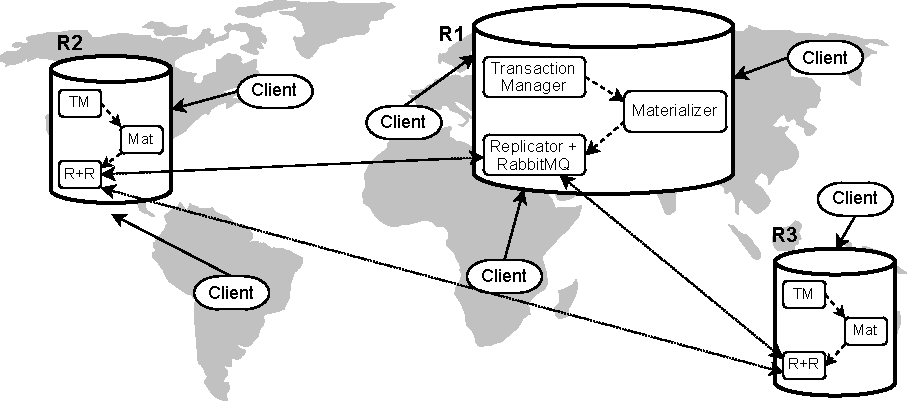
\includegraphics[width=0.85\linewidth]{PotionDBArch}
	\caption{PotionDB Architecture}
	\vspace{-20pt}
	%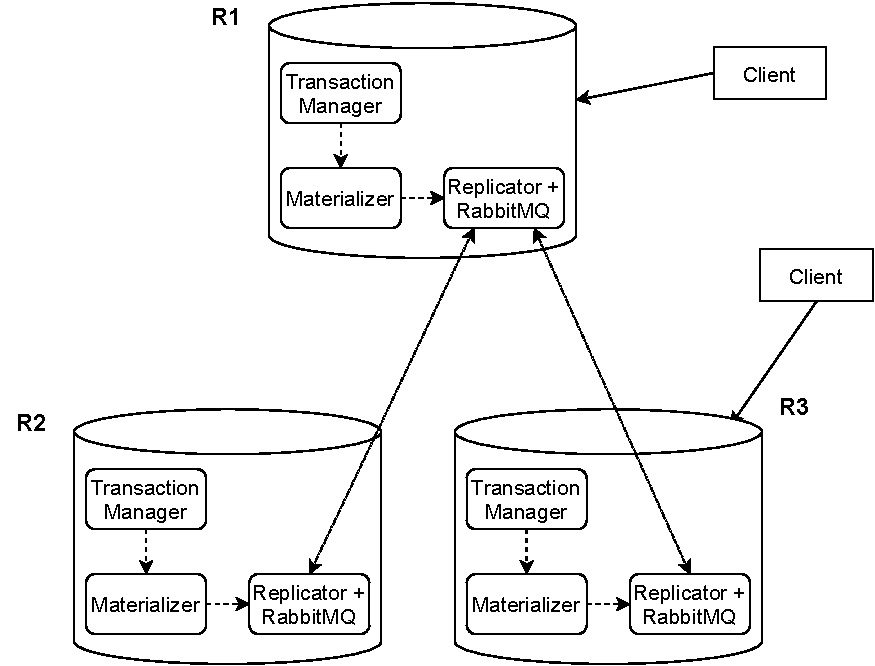
\includegraphics[width=.95\linewidth]{potiondb_architecture}
	%\caption{PotionDB Architecture~\carla{wasted space}}
	\label{fig:arch}
\end{figure}

We designed PotionDB with partial geo-replication in mind.
Thus, we assume PotionDB instances to be spread at different locations across the globe (Figure \ref{fig:arch}).
Each location only replicates a subset of the whole data.
The system administrator has control over where each object, both base objects and views, is replicated.
This allows to account for data locality to ensure fast access to data, while keeping replication and storage costs controlled.
Objects without locality on their access pattern can be replicated everywhere if desired.
%Views can also be partially or fully replicated. %Review: added this to address Rev.A's  comment regarding that views should also be partially replicated in some cases. If needed to cut space, on the phrase "The system adminitrator has control over where each object is replicated", just change to "each object and view are replicated"
We detail this more in Section~\ref{sec:replication}.

%I think details on how transactions work and guarantees do not belong here. So this is OK (but still needs to be explained somewhere).
Clients communicate with the nearest PotionDB location to ensure low latency.
A client's transactions are locally executed in the PotionDB's location the client is connected to.
Updates are propagated asynchronously to other locations.
If a client's transaction accesses objects not locally replicated, other locations with said objects are contacted and involved in the transaction.
We note this should be an exceptional case, not the norm.
We leave further details for Section \ref{subsec:txnproc}.

PotionDB is organized has three modules: the Transaction Manager, the Materializer and 
the Replicator.

The Transaction Manager coordinates transactions execution, executing the TCC protocol presented in Section \ref{subsec:txnproc}.

The Materializer manages the database objects, which encode the type-specific
aspects of PotionDB operation, including rules for conflict-resolution and consistent view 
maintenance for different object and view types. These rules are encoded in CRDT/NuCRDT objects, 
as detailed in Section~\ref{sec:tx:objs}.

The Replicator implements the partial replication protocol detailed in Section~\ref{sec:replication}.
This protocol is type-independent, but it uses information provided by the object in its operation - e.g., 
when a view  is updated, the replicator propagates to other replicas the updates returned by the
view object, which can be an empty set if no updates needs to be propagated.


%The internal architecture of each PotionDB server is inspired by Cure~\cite{cure} and is split into three main components.
%
%First, the Transaction Manager coordinates transactions execution, implementing a transactional protocol (Section \ref{subsec:txnproc}) %which ensures
%ensuring the consistency of reads and updates. %  as well as transactions' atomicity.
%
%Second, the  Materializer stores the objects on their latest version, alongside the necessary data to generate previous versions when necessary.
%Garbage collection ensures data related with versions that are too old is eventually discarded.
%%Garbage collection ensures data to generate versions that are too old is eventually discarded.
%%Garbage collection keeps the amount of metadata in check.
%\nuno{André: o que é que esta última frase quer dizer?}
%%O meu objectivo era mencionar que temos um mecanismo de GC que apaga os dados relacionados com a reconstrução de versões que já não são relevantes (versões muito antigas)
%
%Third,  the Replicator ensures that committed transactions are replicated asynchronously to other PotionDB instances.
%It is also responsible for receiving remote transactions and forwarding them to the Transaction Manager for local execution.
%%The replication component is aware of each instances' replication scheme, ensuring each one only receives updates for objects it replicates. 
%Further details are presented in Section~\ref{sec:replication}.


%=========================================================================================
%=========================================================================================
%=========================================================================================
%=========================================================================================



\section{Transaction and replication protocols}
\label{sec:transactions}

This section presents the 
%underlying 
protocols used to maintain the state of objects
and execute transactions with TCC in PotionDB. 
%The transaction processing and replication
%algorithms are an adaptation of Cure protocols~\cite{cure} to partial replication.

\subsection{Objects}
\label{sec:tx:objs}

PotionDB stores two types of CRDTs: common CRDTs~\cite{crdt} and non-uniform CRDTs (NuCRDTs)~\cite{Cabrita17Nonuniform}, 
which encode the type-specific aspects of PotionDB operation.
%We now explain the guarantees and uses of each type of objects.

\noindent
\textbf{CRDTs.} CRDTs are replicated objects that are guaranteed to converge
after applying the same set of operations. In particular, PotionDB uses operation-based CRDTs,
in which the convergence of replicas is guaranteed if operations are causally applied.
% respecting causality.  
This is the case in PotionDB, as a valid transaction serialization must respect the happens-before
relation, thus guaranteeing that PotionDB replicas converge.
%, i.e., the causal order.

Our prototype supports the following CRDTs: last-writer-wins register, for storing opaque values;
add-wins set, for sets where adding an elements wins over concurrent removals;
add-wins map, for maps of values;
counter, for numbers that accepts concurrent increments and decrements;
average, for maintaining the average of values added to this object;
and an integer register, that keeps the max/min value registered. %Andre: added max/min register, as it is used to implement max() and min() efficiently.

\noindent
\textbf{NuCRDTs.} Non-uniform CRDTs~\cite{Cabrita17Nonuniform} are CRDTs that guarantee that in a quiescent state, 
the \emph{observable state} of all replicas is the same. 
Two observable states are defined as equivalent iff, for each possible read operation, the result is equal when executed on either state.

Unlike normal CRDTs, in NuCRDTs, during the replication process, it is only necessary to propagate
updates that may affect the observable state. For example, consider a maximum object with a \code{insert(n)} and 
\code{getMax()} operations. An \emph{insert} executed in a replica only needs to be propagated 
to other replicas if the inserted value can be the new maximum. 

NuCRDTs allow to save on both replication, processing and storage costs, as not all updates need 
to be replicated and applied everywhere.
In PotionDB, we support the following NuCRDTs~\cite{Cabrita17Nonuniform}: 
\begin{inparaenum}[(i)]
\item maximum and minimum objects, for storing the maximum or minimum of the objects added to the object;
\item top-K, for storing the K entries with largest values;
\item top-K counter, for storing the K (key, value) entries with largest values, where the value
can be updated by issuing increment/decrement operations.
\end{inparaenum}
NuCRDTs can be used directly by applications, but are more commonly used for supporting 
views, as detailed in Section~\ref{sec:views_for_apps}.

\nuno{Dar mais detalhes de como funcionam?}

As proposed by Cabrita et. al.~\cite{Cabrita17Nonuniform}, by not propagating all operations, in some cases, 
a NuCRDT may temporarily expose an incorrect state.
Consider the maximum NuCRDT. Each replica keeps only the maximum element and 
the elements that were inserted locally. If the maximum NuCRDT has a \code{remove(n)} operation,
when the maximum element is removed in some replica, the replica may not have the new maximum,
as it may have been inserted in some other replica.  
All replicas of the maximum NuCRDT eventually 
converge to the new maximum value, as every replica will propagate the local maximum element after receiving the 
remove operation, guaranteeing that all replicas will receive the new maximum.

Tu support views in PotionDB, we had to extend existing NuCRDTs specifications
in three ways.
First, top-K objects, instead of keeping only the value of the element,  keeps multiple
attributes for each element, as needed for storing a complete view entry. An application can update
the value used for establishing the top elements using a set operation (in top-K) or an increment/decrement 
(in a top-K counter). Other attributes can also be updated (as in a map CRDT). %Andre: Rev 370B complained that "this sentence is rather obscure" but I think it's okay like this. If not, just say it is updated together with the set or increment/decrement (which is how it is done).




%By not propagating all operations, in some cases, a NuCRDT may temporarily expose an incorrect state.
%Consider the maximum NuCRDT.  Each replica keeps only the maximum element and 
%the elements that were inserted locally. If the maximum NuCRDT also includes a \code{remove(n)} operation,
%and the maximum element is removed in a given replica, the replica might not have the new maximum element,
%because it might have been inserted in some other replica.  All replicas of the maximum NuCRDT eventually 
%converge to the maximum value, as every replica will propagate the local maximum element after receiving the 
%remove operation, guaranteeing that all replicas will receive the new maximum value.
%
%
%NuCRDTs can be used directly by applications, but are more commonly used for supporting 
%views, as detailed in Section~\ref{sec:views_for_apps}.
%
%
%Our work extends the NuCRDTs specifications proposed by Cabrita et. al.~\cite{Cabrita17Nonuniform}
%in three ways to make them practical for PotionDB.
%First,  a top-K object,  instead of keeping only the value associated with an element,  keeps multiple
%attributes for each element, as needed for storing a complete view entry. An application can update
%the value used for establishing the top elements using a set operation (in top K) or an increment/decrement 
%operation (in a top-K counter).  Other attributes can also be updated (as in a map CRDT). %Andre: Rev 370B complained that "this sentence is rather obscure" but I think it's okay like this. If not, just say it is updated together with the set or increment/decrement (which is how it is done).
%
%%\carla{I don't understand the next paragraph!}
%%As such, a top-K object consists in a set of CRDT maps (rows) with two special elements - the key of the 
%%row and the ordered value used to select the top rows.
%%An application can update the ordered value associated with a key by issuing a set value operation in top-K objects
%%and increments/decrements in top-K counter objects. Other elements can also be updated, given the key of the
%%row, with the operations of the data type.% associated with the row element.
%% \andre{In the implementation, a Top-K entry is a key, value and "an array of bytes" (so, not other CRDTs inside the Top-K). Should we change the text to reflect that?}


%Second, we extend NuCRDT to include information that allows a replica to know if it might be exposing incorrect results. 
%This information consists in the timestamps of transactions that could cause the anomaly - e.g. in our maximum NuCRDT, 
%this is the timestamp of the transaction with the \emph{remove} operation that deleted the previous maximum. 
%Given this information, and knowing the updates that replicas have seen (which is maintained by PotionDB), 
%a replica knows that no anomaly can occur if the operation has been seen by all replicas, 
%which would have triggered replicas to send operations relevant for the observable state, if any.
 
Second, we extended NuCRDTs to maintain a larger observable state to 
reduce the cases in which a replica may be exposing incorrect results - e.g. 
the maximum NuCRDT maintains the two largest elements, guaranteeing that replicas have 
the new maximum if a single remove is issued.
In most practical situations this guarantees that replicas have the correct values - e.g. 
a Top-10 object that keeps the largest 20 elements exposes no anomaly unless
more than 10 concurrent removes of top elements occur, which is very unlikely in practice.

Third, we extend NuCRDTs to include information to know if it might be exposing incorrect results. 
This information consists in the timestamps of transactions that could cause the anomaly - e.g. in the maximum NuCRDT, 
the transactions that \emph{remove} the maximum.
Knowing the updates that replicas have seen (which is maintained by PotionDB), 
a replica knows that no anomaly can occur if the problematic operation has been seen by all replicas, 
which would have triggered replicas to send operations relevant for the observable state, if any.
PotionDB uses this to block reads, as detailed in Section~\ref{sec:replication}.

%In NuCRDTs, when such operations is received by a replica, it sends operations relevant for the observable state to other replicas, 
%if any - e.g. the new maximum in the maximum NuCRDT. Thus, a replica knows it has the correct value when it has the information
%that the problematic operation has been seen in all replicas, which can be verified using information maintained in PotionDB.
%This is used in PotionDB to block reads, as detailed in Section~\ref{sec:replication}.



\subsection{Sharding}
\label{subsec:sharding}

PotionDB adopts a sharded model, where objects replicated in a location are 
split into multiple shards. For durability, each shard could be replicated in multiple
servers \cite{paxos,raft}. %\cite{paxos,raft,chainreplication}.
In each server, a shard has a dedicated thread, adopting an approach used in other
database systems, such as H-Store~\cite{h-store}. This avoids using locks when 
accessing objects, simplifying the implementation and avoiding issues 
as lock contention.


\subsection{Transaction processing}
\label{subsec:txnproc}

The generic transaction processing and replication protocols guarantee that clients access
TCC snapshots and replicas receive relevant updates. PotionDB relies on the type-specific 
information provided by objects for different semantics.

\subsubsection{Metadata}
\label{subsec:metadata}

%Andre: Rev 370B suggested we using, instead of "global" and "local" clocks, a "replica" and "shard" clocks. Should we change that (i.e., does it actually make it more clear?)

Let $L_1$,..., $L_n$ be the set of locations in the system. 
Each location $L_j$ keeps a global vector clock $\mathit{vc}_G$, with one entry for each $L_k \in L_1,..., L_n$.
This clock represents the latest snapshot available in $L_j$, summarizing the transactions integrated in the snapshot.
Each shard $\mathit{sh}_i$ also keeps a local vector clock $\mathit{vc}_i$, with its 
latest snapshot, which may be different 
from $\mathit{vc}_G$.
Any shard can access the server's physical clock, $\mathit{pc}$.

A transaction $t$ has an associated read vector clock, $t\!.\mathit{rc}$,  that represent the snapshot
to be read by the transaction. On commit, a transaction is assigned a commit clock, $t\!.\mathit{ct}$, consisting in a 
pair (timestamp, location identifier).  A transaction with commit clock $(n,r_i)$ is in snapshot $\mathit{vc}_G$ iff
$\mathit{vc}_G[r_i] \geq n$.

%Andre: added the word "also" to address Rev 370B's comment. In the code, the HLC and vci are mixed together... our vci just use the HLC logic to generate the next timestamp. But technically it's as if we have both I suppose.
Each shard also has an hybrid logical clock (HLC)~\cite{hlc} to assign timestamps. An HLC uses the 
physical clock to generate the next timestamp, unless the physical clock is smaller than a timestamp
previously generated/observed. In this case, it returns this value plus one. 
This guarantees that timestamps generated are monotonically increasing.
%Different shards may concurrently generate the same timestamp - in this case, the shard's id is used to break the tie.
%In fact, any monotonically increasing clock would suffice for implementing $\mathit{pc}$.

Each shard $\mathit{sh}_i$ also maintains a list of prepared transactions, $\mathit{prep_i}$, and a list of commits on hold, $\mathit{hold}_i$.
%While we leverage on physical clocks for our protocols, the correctness of our protocols is independent of the skew of physical clocks between servers.


\subsection{Transaction processing}
\label{subsec:txnproc}


A client executes a transaction by interactively contacting the 
Transaction Manager (TM) in a PotionDB server.
%
When the TM receives a \emph{begin} operation, it chooses the latest snapshot available,
$\mathit{vc}_G$, as the snapshot 
the transaction will access.

For an update operation, the TM asks the Materializer to execute the update in
a private copy of the object for the transaction. For a read operation, 
the TM asks the Materializer to execute the read in the private copy - if no 
update has been executed before in the object, a shared copy with the version 
of the transaction snapshot is used. We represent by $t.WS$ and $t.RS$ the update 
and read sets of transaction $t$.

When the TM receives a commit, it needs to assign the commit timestamp to the transaction. 
For assigning the commit timestamp, the TM runs a two phase protocol with the shards of the objects
updated in the transaction. 
\andre{shouldn't it be named "two phase commit protocol"?}

In the first phase,  the TM sends a \emph{prepare} message to all shards in $t.WS$.
A shard $\mathit{sh}_i$ replies with a timestamp proposal, $(n,i)$, where $n$ is the timestamp
generated by the shard's local HLC and $i$ is the shard identifier. Additionally, the shard adds the information
about the transaction, including the proposed timestamp, to the list of locally prepared transactions, $prep_i$.

The TM collects the replies and sets the commit timestamp of the transaction,  $t\!.\mathit{ct} = (\mathit{mts}, j)$,
with $\mathit{mts}$ the largest received timestamp, and $j$ the 
location identifier.
A commit message is sent to all shards in $t.WS$ with the commit timestamp.

When receiving a commit message for transaction $t$, a shard proceeds as follows.
First, it checks if the commit can be applied, by verifying that no prepared transaction or commit on hold have a 
smaller timestamp.
If so, updates from $t$ are marked as committed and the shard's local vector clock $\mathit{vc}_i[j]$ is 
updated with $t\!.\mathit{ct}$. 
%From this point, the Materializer of the shard will generate versions of the object that
%include the committed updates.
Otherwise, the commit is queued to be applied later, as other transactions may commit with a lower
$\mathit{ct}$ than $t\!.\mathit{ct}$.
In either case,  the transaction is removed from $\mathit{prep}_i$. If $t$'s proposed value was the lowest, 
then the Materializer verifies if any commit on hold can now be executed.

The client is informed of the commit as soon as all shards in $t.WS$ acknowledge the commit message, even if 
some shards queued the commit.
When all shards apply the commit, $\mathit{vc}_G$ is updated to include $t\!.\mathit{ct}$.
This promotes freshness, as new transactions will always use the latest committed snapshot.
 %Additionally, the TM sends information to update the global vector clock to
%include the timestamp of the committed transaction.
%Updating the local entry of the global vector clock with the timestamp of committed transactions immediately
%promotes freshness, as new transactions will always use the latest committed snapshot.

However, some shards (not involved in the committed transaction) 
may have transactions to commit with smaller timestamps. 
If a transaction that starts in the most recent snapshot issues an operation on $o$ in a shard that has
pending transactions with smaller timestamps, the operation needs to block if there is a transaction prepared or on hold 
that modified $o$. 


%However, this raises a problem, as some shards (not involved in the committed transaction) 
%may still have transactions to commit with smaller timestamps. 
%If a transaction that starts in the most recent snapshot issues a read (or update) operation on object $o$ in a shard that has
%pending transactions with smaller timestamps, the operation needs to block if there is a transaction prepared or on hold 
%that had modified $o$. 

%Andre: added this paragraph to clarify a situation brought up by Reviewer 370B. In our reply, we mentioned this was unclear so... I explained it here. The question started with: "In fact from the text in this section, I do not understand how txs never end up with the same commit timestamp"
It is possible that two transactions end up with the same $t\!.\mathit{ct}$.
This is not problematic, as a new transaction $\mathit{t}_\mathit{new}$  in a shard first checks if the lowest timestamp in $\mathit{prep}_i$ is lower or equal than $\mathit{t}_\mathit{new}$'s read timestamp for the local replica - if this happens, $\mathit{t}_\mathit{new}$ waits until no such timestamp exists in $\mathit{prep}_i$.
In practice, this is unlikely as nanoseconds are used for time. %IMPORTANT NOTE: while we do not evaluate directly this effect in our experiment, no considerable impact from this is observable (e.g., no considerable latency spikes).


\noindent
\textbf{Operations on objects not locally replicated.}
%\label{subsec:operationsNonLocal}
The protocol presented so far is basically the Cure~\cite{cure} protocol for providing TCC with full replication.
We now show how we extended this protocol to support partial replication and NuCRDTs.
%Unlike the setting for which Cure was designed, PotionDB is partially replicated and a transaction 
%may access an object $o$
%%that is 
%not locally replicated.
%%, $L_i$. 
%Extending Cure to support this case was simple. 

When an operation is executed in an object $o$ that is not locally replicated, 
the shard $L_i$ that should hold $o$ fetches 
a copy of the object from a remote replica. The version
requested is that
of the transaction snapshot,  $t\!.\mathit{rc}$ ignoring the entry for the current location.
%It is important to ignore the current location to guarantee a quick reply. 
%Otherwise, as updates are propagated asynchronously, the remote replica would need to wait to
%receive all transactions from $L_i$ reflected in the transaction snapshot before returning a copy
%of $o$.
After receiving the copy of the object, the shard will apply any updates previously performed to $o$ locally. Typically,
there will be no updates, as $L_i$ does not replicate $o$.
After this, the transaction accesses $o$ as any other locally replicated object. When the transaction commits, 
the updates to $o$ are propagated in the context of the transaction.

\noindent
\textbf{Reads on NuCRDTs.}
As mentioned, NuCRDTs may temporarily expose 
incorrect results when an operation $op$ changes the set of relevant operations.  
As explained, PotionDB is able to detect this situation, which is expected to be rare. 
%maintains information for a replica to know if this is the case 
%and
%it is expected to be a rare situation. \andre{Shouldn't we mention again we have mechanisms to make this situation even more rare to happen? (e.g., maintaining a top of double the size.)}
Applications may select two behaviors when they start a transaction.
First, to ignore potential anomalies and immediately execute the read in the local replica.
This guarantees fast replies at the cost of potential anomalies. 
%
Second, to strictly enforce TCC. In this case, the read blocks until the replica gathers 
information that no relevant operation is missing. This requires receiving information from
all replicas that $op$ was performed and all new relevant operations, if any, have been
received. This is explained in the context of the replication process.
% and explained later.

\noindent
\textbf{Triggers.}
%\label{subsec:triggers}
PotionDB has an after update trigger mechanism that can be associated with 
objects in a bucket or container.
When a transaction executes at the initial replica, after an update, the
trigger runs and it may issue reads and updates to the same or other objects.
These updates are committed and propagated to other replicas
as part of the transaction.

Triggers can be used by applications for any purpose, but its primary goal is to support
incremental view maintenance.%, as detailed in Section~\ref{sec:views_for_apps}.
%In the next section


\subsection{Replication}
\label{sec:replication}

Buckets are the unit of replication in PotionDB.  Each location decides which buckets to replicate.
In our e-commerce example, there is a bucket for 
the customers of each online store.  The container \emph{customers} includes all customer buckets.
The EU customers bucket is  replicated in the EU location and
in one or more additional locations for fault tolerance.

PotionDB adopts operation-based replication, with transaction updates 
being propagated to other replicas. To be more precise, an update
executed in a CRDT generates an \emph{effects} operation that is
propagated and applied in relevant replicas. We start by describing how the replication process
guarantees that transaction updates are propagated to all relevant locations. In the end, 
we discuss the special case of NuCRDTs.

When a transaction commits at a shard, the shard sends its part of the transaction to the replicator.  
Given how transactions are committed at a shard, it is guaranteed a shard sends the transactions
ordered by commit timestamp.
If the shard processes no transaction for some time, it notifies the replicator that there are
no parts of transactions for the shard until the current timestamp, obtained from the shards' HLC.

The replicator processes the parts of transactions received from shards in timestamp order. 
For each transaction, the replicator groups and repartitions the transaction's updates, 
one for each updated bucket. The new parts are queued 
for replication in each bucket, being propagated in order to all locations that 
replicate the bucket. 
A location has a logical stream of updates for all buckets the location replicates
and for the buckets that a local transaction has updated an object.

The replicator integrates remote transactions as follows.
A replicator subscribes to the logical streams of updates for the buckets it replicates from all other 
locations. For the logical streams of each location, it processes transaction parts in timestamp order.
For a given timestamp, the replicator groups the parts of the transaction $t$ and verifies if the causal dependencies 
of $t$ are satisfied by checking whether $t.rc \leq \mathit{vc}_G$.
If true, the replicator 
%repartitions the transaction according to
%the local shards and 
forwards the
% transaction 
transaction updates to the local shards for execution. 
After all shards involved in $t$ end, 
%that they have executed their part of the transaction,  
the global
vector clock is updated to include the timestamp of $t$. If false, then some transactions
from other locations need to be applied before $t$. So, the replicator continues by processing
the logical streams from other locations.
Furthermore, the replicator piggybacks to other locations the information about locally executed transactions.
For fault-tolerance, a location forwards updates from a failed
location to other locations.

\textbf{Support for NuCRDTs.}
\label{subsec:nonuniform}
%Note: we do not really guarantee causality when considering non-uniform CRDTs. How should we handle this? Do we mention this in the paper? Or maybe mention how we could "fix" this?
NuCRDTs use a non-uniform replication approach~\cite{Cabrita17Nonuniform}, in which some 
updates might not need to be propagated, as explained in Section~\ref{sec:tx:objs}.
Not immediately propagating some updates is straightforward, as, when executed locally, 
an update operation may produce a null \emph{effect} update if there is no
effect in the observable state.

%as update operations generate 
%the \emph{effect} update to be remotely propagated,
%% to other replicas,
%If an update operation has no
%effect in the observable object state, hence does not need to be propagated, 
%the update operation just generates a null effect.

In NuCRDTs, the execution of an operation $op$ may make a previous local operation  $op_{p}$
relevant, requiring $op_{p}$ to be propagated to other replicas  
(e.g.  \code{remove(n)} in the maximum NuCRDTs makes the insertion of the second
maximum element relevant). There are two cases to be considered.
%
First, when $op$ executes in the initial replica, the effect of
$op$ will include also the effect of $op_{p}$. As the combined effects are propagated and applied in 
the context of the same transaction, no anomaly is generated.
%
Second, when the now relevant $op_{p}$ operation was executed in  
another replica. This is handled by replication process as follows.  When a location receives
the replication stream from other replicas, it executes the received \emph{effects} in the objects' local copy.
For NuCRDTs, the execution of an \emph{effect} operation may generate additional 
\emph{effects} - in our example, the execution of the \emph{effect}s of $op$ would generate
the effects of $op_{p}$. These extra effects are propagated to other replicas
%to other locations 
along with the 
information that $op$ has been executed.

%Our transactional and replication protocols ensure that objects' states evolves monotonically.
%Clients keep a vector clock representing the latest database snapshot observed, allowing clients to see a consistent state even if they migrate to a different replica.
%We detail this further in Section \ref{sec:transactions}. %Andre: added this to address Rev 370B.


\section{Views and Experience}
\label{sec:views_for_apps}

We now discuss how PotionDB supports materialized views.
%, by using PotionDB
%objects and triggers generated from the view specification. We also discuss
%and our experience in defining views for TPC-H queries. 

\subsection{Generated objects and triggers}
\label{subsec:generated_view}

We now outline how PotionDB, given a view specification, generates the 
%right 
objects to hold the view's data and its updates. % the views.
%For the sake of brevity and simplicity, we do not dive deep into the details of the algorithm, instead showing the intuition behind it.

\noindent
\textbf{Generated objects:}
The objects used for storing the view's data depends on the type of query. 
%If the query has no  \emph{limit} clause and includes either no aggregation or an aggregation of type sum (or similar, such as count or average), the view will be stored in a map CRDT, where the full materialized view is maintained. 
%If the query has a  \emph{limit} clause or includes an aggregation of type maximum (or minimum),
%the top-K is used.
%If the query has a  \emph{limit} clause and an aggregation of type sum (or similar, such as count or average),
%the top-K counter is used.
If the query has no  \emph{limit} clause and includes either no aggregation or an aggregation of type sum (or similar, such as count or average), maximum or minimum, the full materialized view will be stored in a map CRDT. 
If the query has a  \emph{limit} clause and no aggregation, or an aggregation of type maximum (or minimum), the top-K is used.
If the query has a \emph{limit} clause and an aggregation of type sum (or similar), the top-K counter is used.
In any case, the elements of the view are maps with multiple columns, one for each
attribute specified in the  \emph{select} of the view definition.  

%For a given view, one or multiple objects are used - 
For a view that includes variables, multiple objects are used,
one for each possible value of the variables. 
In the top sales example of Figure~\ref{fig:viewtopsales}, one top-K counter
object is created (as needed) for each month of each year, and its PotionDB key includes
the name of the view plus the month and year.  The top-K counter will have a set
of entries, each one with the identifier of a product and the total sales of the product. The entry
could have additional information, such as the 
description of the product if that was defined in the view.

\noindent
\textbf{Generated triggers:}
PotionDB generates triggers to update 
the contents of view objects,
%of the view, 
as base objects are created, updated or deleted.
% (referred simply as updates). 
The triggers will be set for the container (or buckets) specified in the \emph{from} clause of the view definition.
If a \emph{where} clause is included, updates to objects that do not match the 
defined condition will be ignored.

As a view may be composed by multiple objects, it is first necessary to 
determine which view object must be updated. This is achieved from the view definition 
and the values in the updated base object - in our running example, 
from the date of a sale, it is immediate to know which view object
must be updated.
The exact operation generated to update the view object depends on the type of view object, 
but it consists in applying the same update performed in the base object to the 
corresponding view entry map.
For example, consider the creation of a new sale for product $P$, with the value $v_P$. 
In this case, the top-K counter of the month and year of the sale is updated by 
incrementing the total value of sales for $P$ by $v_P$. 
The underlying functionality of top-K counter guarantees that the updated entries
will be propagated to other replicas when necessary, and that replicas keep the correct top-K
elements.

\subsection{Developer-defined views}
\label{subsec:programmer_view}

A developer can create views by defining the objects to maintain the view's data and the
triggers to update these view objects.
%When the PotionDB's view language is not sufficient for defining the views an application needs, 
%a developer can define objects to maintain the view's data and the
%triggers to update these view objects.
The top-K and top-K counter NuCRDTs include the logic for replicating only the necessary 
updates to maintain in all replicas the top elements for data that is updated using set value 
or increment operations.
When the view does not consist in the topmost elements, the Map CRDT can be used.  
Aggregations defined in the views - e.g. sum, maximum - are supported by using CRDT and NuCRDT 
objects, such as the counter CRDT and maximum NuCRDT.
After defining the objects to be used, the application should define the triggers that (populate and) 
update the view objects. 


\subsection{TPC-H in PotionDB}

We now describe our experience applying our 
model to the queries defined in TPC-H.

\subsubsection{Data model}
\label{subsec:dataset}

TPC-H data is typical of an e-commerce service with tables storing information about customers, suppliers, parts (products), orders, 
countries and regions (continents).
Two extra tables represent associations: partsupply and lineitem represent, respectively, a part provided by a supplier
and a product sold in an order. 

As the dataset includes countries and regions, it is straightforward to define a partial replication strategy. 
For each table that will be partially replicated, we define a bucket for each region and a container including all these buckets.
For tables that are fully replicated, there is a single bucket and container. 
We do the following mapping from tables to buckets: 
\begin{inparaenum}[(i)]
\item Customers, suppliers, nations and regions have 
%a nation or 
region directly
associated with it, which is used to select the bucket to use;
\item Orders are stored in the region of the customer;
\item Partsupplies are stored in the supplier's region;
\item Lineitems are stored in the customer's and supplier's region, as this information is relevant for both.
\item Parts are used across the globe, so they are stored in a single bucket to be fully replicated;
\end{inparaenum}

Each table row is stored as a map CRDT, with the key of the row (e.g. the identifier of a customer or the combination of part key and supplier key for partsupply) used as the key in PotionDB's object identifier. 
Each column is a CRDT - e.g. the counter CRDT is used for numbers that are updated using numeric operations and the
LWW register is used for strings and other numbers.
When useful, we de-normalize the data model (as it is common in NoSQL databases). 

\subsubsection{Views}
\label{subsec:views_for_queries}

%%Should we make it clear somewhere our PotionDB prototype does not have this specification implemented/supported?
%Given a recurrent query, the application developer can specify one or more views that hold the necessary data 
%to answer the query directly, without requiring to read multiple objects, do joins or other resource-consuming processing.
%An important aspect to consider, when devising the views, is that some queries have parameters and other don't.
%For example, if the goal is to know top seller product of all times (or in a game the leaderboard of the game), the query 
%will have no parameter and the view will
%be exactly the same as the result of the query. However, if the query to be performed by the application has 
%parameters, the view needs to include all values needed to answer the query with the different possible values. 
%The example of top sales view presented in Section~\ref{subsec:interface} exemplifies this, where the view includes
%the top sales products for each month - an application will query the view to get the information for a given month.
%
%\nuno{Qual o objetivo do próximo examplo - mostrar como fazer? neste exemplo não sei bem como especificar...}
%As in relational databases, the challenge is, thus, to specify the right views for the application's queries.
%PotionDB's view API (Section \ref{subsec:interface}) and its similarities with SQL make this challenge somewhat similar to the one faced when using relational databases.
%PotionDB automatically generates the necessary objects and update rules for the view(s), ensuring views are correctly updated when any base object is inserted/updated/deleted.
%Such inference takes out a considerable burden from the application developer.

We analyzed how to define views in PotionDB for all 22 TPC-H queries.
We now describe the lessons learned. 
%In the next section we present the evaluation of how PotionDB performs on supporting
% different types of queries.

\paragraph{De-normalization.} PotionDB is a key-value store and does not directly support advanced database functionality,
such as joins.  To address this issue, we de-normalize the database whenever necessary.  
The view in Figure~\ref{fig:viewtopsales} is an example of such de-normalization, with
the product name (\texttt{prodname}) stored in the sales record, instead of the product identifier.

\begin{figure}[t]
\small{
\begin{lstlisting}[language=SQL]
CREATE VIEW (Q5, views) WITH REGION == 
ANY (SELECT DISTINCT R_name FROM region) AS
SELECT R_Name, N_Name, SUM(ExtendedPrice * (1 - Discount)) AS Revenue
FROM Lineitem
WHERE C_NationKey == S_NationKey AND R_Name == [REGION]
GROUP BY N_Name
ORDER BY Revenue DESC
\end{lstlisting}}
	\vspace{-10pt}
	\caption{Revenue of local suppliers (Q5).}
	\vspace{-10pt}
	\label{fig:viewlocalsupliers}
\end{figure}


% diferentes tipos de dados
\paragraph{Data types.} Different types of view require different support from PotionDB data types.
Figure~\ref{fig:viewlocalsupliers} shows the view for TPC-H query 5, which computes
for each nation in a given region, the revenue from local suppliers. 
This view uses for each region a map that stores for each nation the sum of the 
revenue for each \texttt{LineItem}. The map of each region is a CRDT map, with the name of the nation mapping
directly to a CRDT counter with the revenue for that nation. When a new \texttt{LineItem} is added (or deleted), 
the corresponding counter is updated. All replicas will have all the values for all nations.

This contrasts with the top sales shown in Figure~\ref{fig:viewtopsales}, that uses a
top-K counter. In this case, whenever a new sale is inserted, the counters associated with the products are
updated, but each replica maintains only a partial view of the top-K object - as explained before, replicas only propagate 
%to all replicas 
the updates for elements that may belong to the top-K.

Finally, some views use top-K objects. Figure~\ref{fig:q18_view} shows the view to 
support TPC-H query 18, which returns the top 100 most valuable orders larger than 
some given quantity.  In this case, a top-K object is sufficient - the difference with a top-K counter is that,
while in the top-K a view entry is completely defined by the value of an order and can be derived 
from the insert (or update) of an order, in the top-K counter, the value of an entry is the result of an 
aggregation over multiple values (in the example, \texttt{LineItem}s of different orders).


\begin{figure}[t]
	\begin{lstlisting}[language=SQL]
CREATE VIEW (Q18, views) WITH QUANTITY == [312..315] AS
SELECT CustName, CustKey, OrderKey, OrderDate, TotalPrice, TotalQuantity
FROM Orders
WHERE TotalQuantity > [QUANTITY]
ORDER BY TotalPrice DESC, OrderDate ASC
LIMIT 100
	\end{lstlisting}
	\vspace{-10pt}
	\caption{Large volume customer query (Q18).}
	\vspace{-10pt}
	\label{fig:q18_view}
\end{figure}


% definição de variáveis
\paragraph{Variables:} As introduced in Section~\ref{subsec:interface}, it is possible to define 
variables in the specification of views. %In some cases, it is important that the view includes information 
%for every possible value of the variables - 
When used, a different object is maintained for each
value of the variable (or combination of values of multiple variables). 
For example, for the view of Figure~\ref{fig:viewlocalsupliers}, there
will be an object for each region and for the view of Figure~\ref{fig:viewtopsales}, there 
will be an object for each combination of month and year.

In other cases, the application will only query the database using some specific values of the
variables. For example, the specification of the TPC-H query 18 states that quantity will be instantiated with values
from 312 to 315. 
Figure~\ref{fig:q18_view} shows how this can be specified in PotionDB, leading to four object, 
one for each value of \texttt{quantity}. Whenever a new
order is inserted (or updated), the four objects might need to be updated.
We note that this situation is common in application, as interfaces often limit the queries a user can 
perform - e.g. hotel reservation applications allow users to check hotels with an average 
rating larger than some predefined values.
%Figure~\ref{fig:q18_view} shows how this can be specified in PotionDB for TPC-H query 18. 
%In this case, four objects will be created, one for each value of \texttt{quantity}. Whenever a new
%order is inserted (or updated), the four objects might need to be updated.

% limitações
\paragraph{Limitations.} 
The language for specifying views in PotionDB has several limitations, including the 
lack of support for joins and sub-queries, and the limited expressiveness in clauses like select and where. 
Supporting full SQL in view definition is not the focus of our work and it is overly complex, as exemplified by the fact that PostgerSQL incremental view 
maintenance extension \cite{ivm} still lacks many SQL features after 10 years of development. 
Our work focus on providing the mechanisms to support consistent views over geo-partitioned data. 
Programmer can always \emph{manually} define a view by selecting the appropriate objects to store the information and 
defining the necessary triggers to update these objects.

%
%compared with support for defining views in relational databases. The main limitations concern the 
%lack of support for joins and sub-queries, and the limited expressiveness in clauses like select and where. 
%This complicates the specification of views for some complex queries and might even make it 
%impossible to use our view definition language.  In this latter case, the programmer can resort to \emph{manually}
%define a view, by selecting the appropriate objects to store the information and defining the necessary triggers
%to update these objects.

%\vspace{-5pt}
\begin{figure}[t]
	\begin{lstlisting}[language=SQL]
CREATE VIEW (Q11_p1, views) WITH NATION == ANY 
(SELECT DISTINCT N_Name FROM nation) AS
SELECT N_Name, Partkey, SUM(Supplycost * Availqty) AS Value
FROM Partsupp
WHERE N_Name == [NATION]
GROUP BY Partkey
LIMIT 1000

CREATE VIEW (Q11_p2, views) WITH NATION == ANY
(SELECT DISTINCT N_Name FROM nation)  AS
SELECT N_Name, SUM(Supplycost * Availqty) AS Value
FROM Partsupp
WHERE N_Name == [NATION]
ORDER BY value DESC
\end{lstlisting}
\vspace{-10pt}
	\caption{Important stock identification query (Q11). %ORDER BY added to answer review.
	}
	\vspace{-10pt}
	\label{fig:q11_view}
\end{figure}

Sometimes it is possible to circumvent the limitations by defining additional views.
For example, TPC-H query 11 finds the suppliers stocks in a given nation that represent a significant percentage of the total
value of available parts in the nation. TPC-H specification uses a having clause with a condition expressed as a subquery.
In PotionDB, we can define view \texttt{Q11\_p2} with the total value for each nation, and view \texttt{Q11\_p1} with 
the top parts for each nation, as shown in Figure~\ref{fig:q11_view}.
%The \texttt{Q11\_p2} view maintains the total value for each nation, while the \texttt{Q11\_p1} view
%maintains the top parts for each nation. 
The result of Q11 is obtained reading the total value for the nation, and using this value for 
filtering the top parts (as some parts may not
reach the percentage ratio specified).


\section{Evaluation}
\label{sec:evaluation}

%\begin{itemize}
%	\item Say that we evaluate PotionDB's performance
%	\item Give a short summary of what we try to access
%	\item Describe the three modes of PotionDB (normal, "partitioned views/Local PotionDB", "single view server/Single PotionDB")
%\end{itemize}


We evaluated PotionDB's prototype to answer the following questions: 
\begin{enumerate*}[label=(\roman*)]
	\item  \label{enum:q1} Can global views over partially geo-replicated data provide better performance than alternative approaches? 	     
	\item \label{enum:q2} Are global views still worthwhile with low latency among servers?
	\item \label{enum:q3} How do different types of views behave? 
\end{enumerate*}

Our prototype was implemented in Go and uses Google's protobufs to serialize/deserialize all data transmitted.

\subsection{Experimental setup}
\label{subsec:setup}

We compare the following alternatives to maintain views:
\begin{itemize}[leftmargin=*,noitemsep,topsep=0pt,parsep=0pt,partopsep=0pt]
	\item \emph{PotionDB}, our proposed approach where all servers replicate the complete materialized view;
	\item \emph{Local}, where each server maintains a local view that includes only the objects replicated in the server - in this case, 
	updates to the view result only from updates to the objects replicated in the server; 
	on reads, it may be necessary to contact multiple servers;
	\item \emph{Single}, where the view is maintained in one server - in this case, a query needs to 
	contact the server that holds the view, if this is not the local server. 
\end{itemize}
The alternative approaches are implemented using PotionDB codebase - in this way, propagation of view updates uses the same underlying mechanisms, but updates are only sent to the appropriate replicas; queries that require accessing views not locally replicated are propagated to the remote server, where the reads are executed and the results returned (as a consequence, in \textit{Local} and \textit{Single}, TCC may be violated).
In Section~\ref{sec:eval:postgrs} we compare our approach with PostgreSQL.

%We evaluate PotionDB using TPC-H's dataset, queries and updates, as well as with micro-benchmarks.
%For the evaluation using TPC-H, we 
We evaluate PotionDB on Grid'5000's \cite{Grid5000}, using TPC-H's benchmark \cite{tpch}, with a scale factor of 1. %Andre: added at request of reviewer 370B.
We modeled the database as discussed in Section~\ref{subsec:dataset} and used data generated by dbgen tool \cite{tpch}.

%Andre: rewrote this whole paragraph to address reviewer 370B asking which queries we choose and for some more clarity.
Unless otherwise stated, our experiments execute TPC-H queries 3, 5, 11, 14, 15 and 18.
This mixed workload has queries ranging from a single table (e.g. Q11) to multi-join (e.g. Q5), limits (e.g. Q18), averages (e.g. Q14), sums (e.g. Q5), 
among other factors. It also includes queries concerning a region or country (Q5 and Q11) and worldwide (Q3, Q14, Q15, Q18) data.
The former lead to \textit{local} views, which aggregate data of a region/country, while the latter lead to \textit{global} views, which aggregate worldwide data. 
Although PotionDB supports views to be partially replicated, in our configuration of \textit{PotionDB}, we replicate \textit{local} views in all replicas.

%Andre: added this last phrase as for some reviewers it is not clear if local views are replicated everywhere. In the TPC-H  benchmarks, in PotionDB (not local/single), even local views are replicated everywhere. This was just because of convenience in implementing the client... so I do not know how to justify it here. Should I just adapt the experiments for Global to only replicate the local views locally?

%In our evaluation we selected some queries to define views, trying to consider queries with different requirements. 
%%For example, while some TPC-H queries concern worldwide data (e.g. query 18 mentioned before), others, \textit{local} queries, concern data of one continent and country (e.g.  queries 5 and 11). The former lead to \textit{global} views, with each entry combining data from all regions, and the latter lead to \textit{local} views, with each entry combining data from a single region. 


We have used 10 machines, with a 2x Intel Xeon Gold 6130 with 192GB of RAM, interconnected with a 10Gbps Ethernet network. 
We have divided the machines in 5 groups,  each one representing a region, with one machine for running the server and one machine for running the clients.  
Data is partitioned as described in Section \ref{subsec:dataset}. 
We have used the Linux \texttt{tc} command to add latency between nodes in different groups, using as reference the latency between AWS instances measured in \cite{AWSLatency} for regions EU (Paris), US (N.Virginia), Canada (Central), Asia (Tokyo) and Middle East (Bahrain). The highest latency is between Tokyo and Paris at 217ms.  
%This distribution does not include data centers in each continent, as there was no information for Oceania - we note that this is less favourable for PotionDB, as in PotionDB queries are always local, while in alternative approaches some queries need to access remote servers. 

For each experiment, we restart the servers and load the initial database. 
Each result is the average of three runs. 
For each configuration, we run experiments with an increasing number of clients. 



\subsection{Performance with geo-replication}

We start by analysing PotionDB's performance in our targeted partially geo-replicated scenario.

\begin{figure}
	\centering
	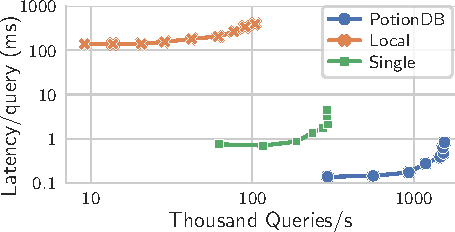
\includegraphics[width=0.6\linewidth]{singleQuery/all_queries_tc}
	\vspace*{-0.85em}
	\caption{Query-only performance of executing all queries.}
	\label{fig:global_local_single_tc}
	\vspace*{-11pt}
\end{figure}%
\begin{figure}
	\centering
	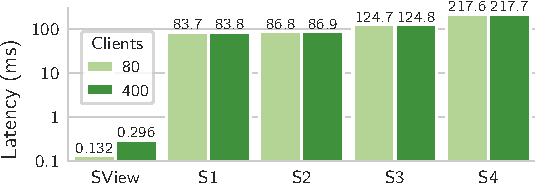
\includegraphics[width=0.72\linewidth]{singleQuery/single_TC_latencies}
	\vspace*{-0.85em}
	\caption{Average latency in \textit{Single}, per server.}
	\label{fig:single_tc_latencies}
	\vspace*{-11pt}
\end{figure}%

\noindent
\textbf{Query performance and benefits of views.}
Figure \ref{fig:global_local_single_tc} shows the results of running all selected TPC-H queries for the three alternative approaches. 
As expected, \textit{PotionDB}'s throughput, latency and scalability are considerably better than alternative approaches, reaching 
1.5 million queries/s with latency under 0.6 milliseconds. 
This results from all queries being local, while in alternative approaches, global queries need to access data from 
remote replicas. In this case, servers end up consuming most of the time managing communications with other replicas, leading 
%not only
to higher latency 
%but also to 
and lower throughput. 

When comparing the results of \textit{Single} and \textit{Local}, the \textit{Single} configuration has much lower latency and higher throughput. This is explained by the fact that clients connected directly to the server that holds the views are very fast and 
end up executing a much higher number of requests than clients in other regions, which experience high latency- this can be 
seen in Figure \ref{fig:single_tc_latencies}, that shows the latency of clients in each region.

To conclude, having global, complete views replicated in every server allows all clients to achieve low latency and high throughput in \textit{PotionDB}, while \textit{Local} and \textit{Single} approaches suffer from comparatively high latency and low throughput.



\begin{figure}
	\centering
	\begin{subfigure}{.49\linewidth}
		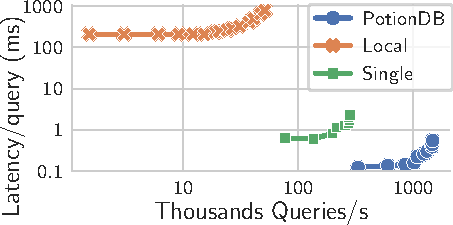
\includegraphics[width=1\linewidth]{singleQuery/q3_latency}
	\vspace*{-10pt}
			\caption{Q3-only (global query).}
		\label{fig:q3_tc}
	\end{subfigure}%
	\hspace*{0.2em}
	\begin{subfigure}{.49\linewidth}
		%\raggedright
		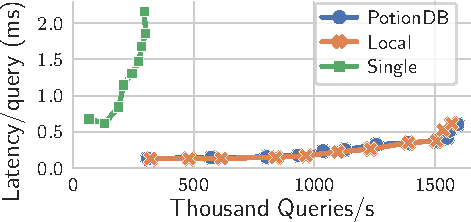
\includegraphics[width=1\linewidth]{singleQuery/q5_latency}
	\vspace*{-10pt}
		\caption{Q5-only (local query).}
		\label{fig:q5_tc}
	\end{subfigure}%
	\vspace*{-10pt}
	\caption{Query performance when executing only Q3 or Q5.}
	\label{fig:q3_q5_tc}
	\vspace*{-10pt}
\end{figure}

%TODO: Effects of query locality or data locality?
\noindent
\textbf{Effects of query locality.}
For better understanding the effects of data locality,  Figures \ref{fig:q3_tc} and \ref{fig:q5_tc} present, respectively, the performance when
executing a single global query (TPC-H Q3) and local query (TPC-H Q5). 
For the global query, the results are similar to the complete workload, the main difference being an increase in latency and reduction in  throughput for the \textit{Local} configuration. In this case this is explained by all queries needing to contact remote servers and results do not include the effects of operations that execute locally.

For the local query, the \textit{Local} configuration performs similarly to \textit{PotionDB}. The reason for this is that, in this case, queries only access the local server that has all necessary information - a client in a region only performs requests for data of that region.
In short, \textit{PotionDB} is efficient for both global and local queries, while \textit{Local} is heavily hindered by latency for any query that is not fully local.

%II have to do these two graphs (I have the necessary data however).
%Here's what those graphs will show.
%
%Graph one: Q3 (global query). PotionDB will scale fine, up to 4.5m ops/s, unnafected by latency (around 0.8ms at 4.5m ops/s). Local PotionDB will be a disaster, with around 210ms latency and up to 70k ops/s. Single PotionDB will get up to around 900k ops/s (1/5th of PotionDB), with around 3-4ms of latency (some effect from added latency).
%
%Graph two: Q5 (local query). PotionDB and Local PotionDB will scale similarly: respectively, 4.1m ops/s and 3.9m ops/s. Both are unaffected by added latency, Local PotionDB even has slightly lower latency. Single PotionDB will have 1/5th of their performance and around 3-4ms latency (i.e., some effect from added latency).
%
%\begin{itemize}
%	\item executing only global queries (Q3) further exacerbates how poorly Local PotionDB performs, due to having to contact all servers for each query. (similar conclusions to the previous section)
%	\item when executing local-only queries (Q5), local PotionDB performs similarly to PotionDB - no redirection of requests is needed (clients only ask for data of their region), thus local PotionDB can efficiently reply to queries with only its local data views. Our solution "does not lose" to the local view solution.
%\end{itemize}

%\begin{figure*}
%	\begin{subfigure}{0.31\linewidth}
%		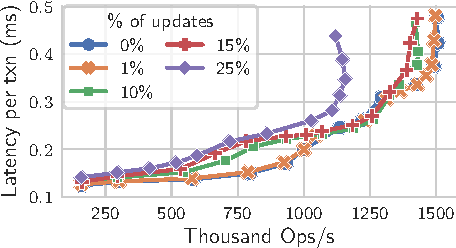
\includegraphics[width=1\linewidth]{singleQuery/upd_rate_global}
%		\caption{PotionDB.}
%		\label{fig:update_rates_global}
%	\end{subfigure}%
%	\hspace*{0.5em}
%	\begin{subfigure}{.31\linewidth}
%		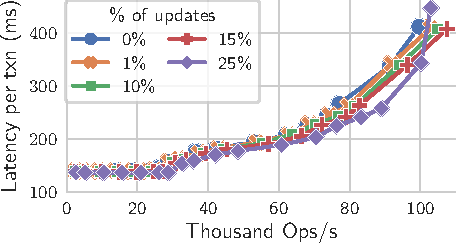
\includegraphics[width=1\linewidth]{singleQuery/upd_rate_local_tc}
%		\caption{Local PotionDB.}
%		\label{fig:update_rates_local_tc}
%	\end{subfigure}%
%	\hspace*{0.5em}
%	\begin{subfigure}{.31\linewidth}
%		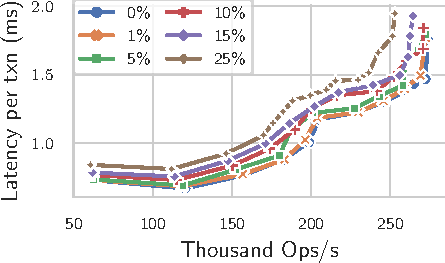
\includegraphics[width=1\linewidth]{singleQuery/upd_rate_single_tc}
%		\caption{Single PotionDB.}
%		\label{fig:update_rates_single_tc}
%	\end{subfigure}%
%	\vspace*{-0.75em}
%	\caption{From left to right, total throughput of PotionDB, Local PotionDB and Single PotionDB with a varying update rate.}
%	\label{fig:upds_tc}
%	\vspace*{-0.6em}
%\end{figure*}
\begin{figure}
	\centering
	\begin{subfigure}{.47\linewidth}
		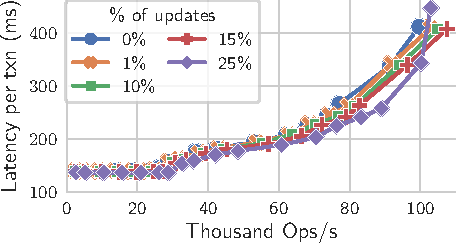
\includegraphics[width=1\linewidth]{singleQuery/upd_rate_local_tc}
	\vspace{-10pt}
		\caption{Local.}
		\label{fig:update_rates_local_tc}
	\end{subfigure}%
	\hspace*{0.2em}
	\begin{subfigure}{.52\linewidth}
		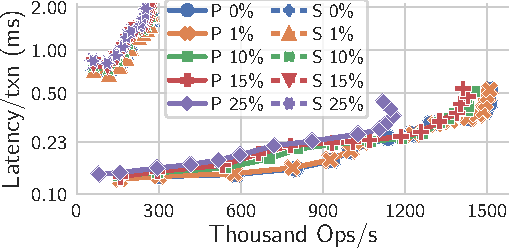
\includegraphics[width=1\linewidth]{singleQuery/upd_rate_tc_global_vs_single}
	\vspace{-10pt}
		\caption{\textit{PotionDB} (P) and \textit{Single} (S).}
		\label{fig:update_rates_global_single_tc}
	\end{subfigure}%
	\vspace{-10pt}
	\caption{Performance with multiple update rates.}
	\label{fig:upds_tc}
	\vspace{-15pt}
\end{figure}


\noindent
\textbf{Impact of updates.}
\textit{PotionDB}'s approach of maintaining a copy of the views in every server imposes additional load on the system
for keeping views updated,  when compared with the \textit{Local} and \textit{Single} approaches. 
In \textit{PotionDB}, a view update needs to be executed in every replica while in the other approaches the view update 
is applied only in a single replica. 

To evaluate the impact of updates we consider workloads consisting in different ratios of updates and queries, with
an update being the transaction that creates a new order, and a query being one of the queries defined in
TPC-H.
% - the 25\%/75\% ratio means that 25\% of operations are updates. 
The results of our experiments
are presented in Figure~\ref{fig:upds_tc}.

%0: 1.511M ops/s, 0.01: 1.517M ops/s,  0.05: 1.46M, 0.1: 1.45M, 0.15: 1.43M, 0.25: 1.157M
%PotionDB has small throughput losses for modest update rates (between 0.1\% and 5.4\% for update rates up to 15\%), while for 25\% it has a significant drop of 23.4\%.
The results show that for \textit{PotionDB}, for 1\% update rate, the impact in throughput is unnoticeable, when compared with a read-only workload.
The throughput starts decreasing as the ratio of updates increases - 4\% drop for 10\% updates and 23.4\% for 25\% of updates.
The reduction in performance results not only from the fact that view updates need to be executed in all replicas, but also because 
updates are inherently slower as the commit of a transaction requires coordination among the multiple shards involved in the transaction. 
Note that queries' latency only raises slightly as, in practice, they seldom need to wait for updates.
%25\%: 0.273304; 0\%: 0.245562
For instance, at \textit{PotionDB}'s maximum throughput for 25\% updates, the query-only latency is 0.273ms, which compares to 0.246ms for 0\% of updates.

%To execute an update transaction, shards have to synchronize to apply the commit protocol (Section \ref{subsec:commit}) - thus, as the update rate gets higher, this synchronization happens more often, potentially making other queries/updates wait.
%This synchronization, as well as multiple updates being in the same transaction, is why update transactions have higher latency than queries, as seen on Figure \ref{fig:update_latency}.
%We note however that in practice queries seldom have to wait for updates unless the server is saturated, as can be seen in Figure \ref{fig:query_latency}.
%The main observable difference in query latency is the latency at the middle of the throughput raising earlier.
%We believe this may be due to network artifacts that lead to latency raising slightly when using over a certain amount of bandwidth - since update transactions have many updates, this threshold is reached with less clients. %TODO: This is... not really a good explanation. Sigh

\textit{Local} throughput improves as the ratio of updates increase. This results from reporting
the number of executed operations with create transactions that includes multiple updates. 
The overhead for executing a transaction (messages for starting and committing a transaction) is paid
only once for multiple operations\footnote{In \textit{PotionDB}, if a transaction includes 5 queries/transaction the maximum throughput 
goes to 4.83M op/s (with latency of 0.68ms), when compared with 1.5M ops/s with (with latency of 0.37 ms) for one query per transaction.}.  
Moreover, update transactions contact less servers (as updates propagate asynchronously and 
orders are local - 50\% \footnote{This does not occur on the original TPC-H dataset, 
whose orders' items are random. This modification adds locality to orders, which is more realistic for 
an e-commerce scenario and helps \textit{Local} more than \textit{PotionDB}.}- or refer few regions). 
This leads to a slightly lower average latency \mbox{with higher update rates.}

%fig:update_rates_single_tc
\textit{Single} configuration has throughput losses comparable to \textit{PotionDB}'s, except for 25\% updates where the drop in throughput is smaller 
than \textit{PotionDB}'s due to not having to replicate view updates.
However, even for 25\% updates, \textit{Single}'s throughput is less than 1/4 of PotionDB.

In summary, %PotionDB scales well with modest update ratios, which are common in practice.
PotionDB provides scalable TCC viewsm answering complex global queries in sub-millisecond time.
%Moreover, updates in PotionDB are unaffected by latency between servers.


%Two to three graphs: global with updates, local with updates, (optionally) single with updates. I have to modify the graphs to not count with updates for the views.
%
%Note: both graphs below still account for view updates on their throughput. 
%View updates account for around 2/3rd of the update count.
%
%%Graph global: higher update rates mean lower max throughput and a bit higher latency (e.g., 0\% updates starts at 0.3ms, 100\% starts at 0.5ms). The old graph of this one (still counting with view updates) is on Figure \ref{fig:(new)update_rates}.
%%Graph global: Check Figure \ref{fig:(new)update_rates}
%
%\begin{figure}[h]
%	\centering
%	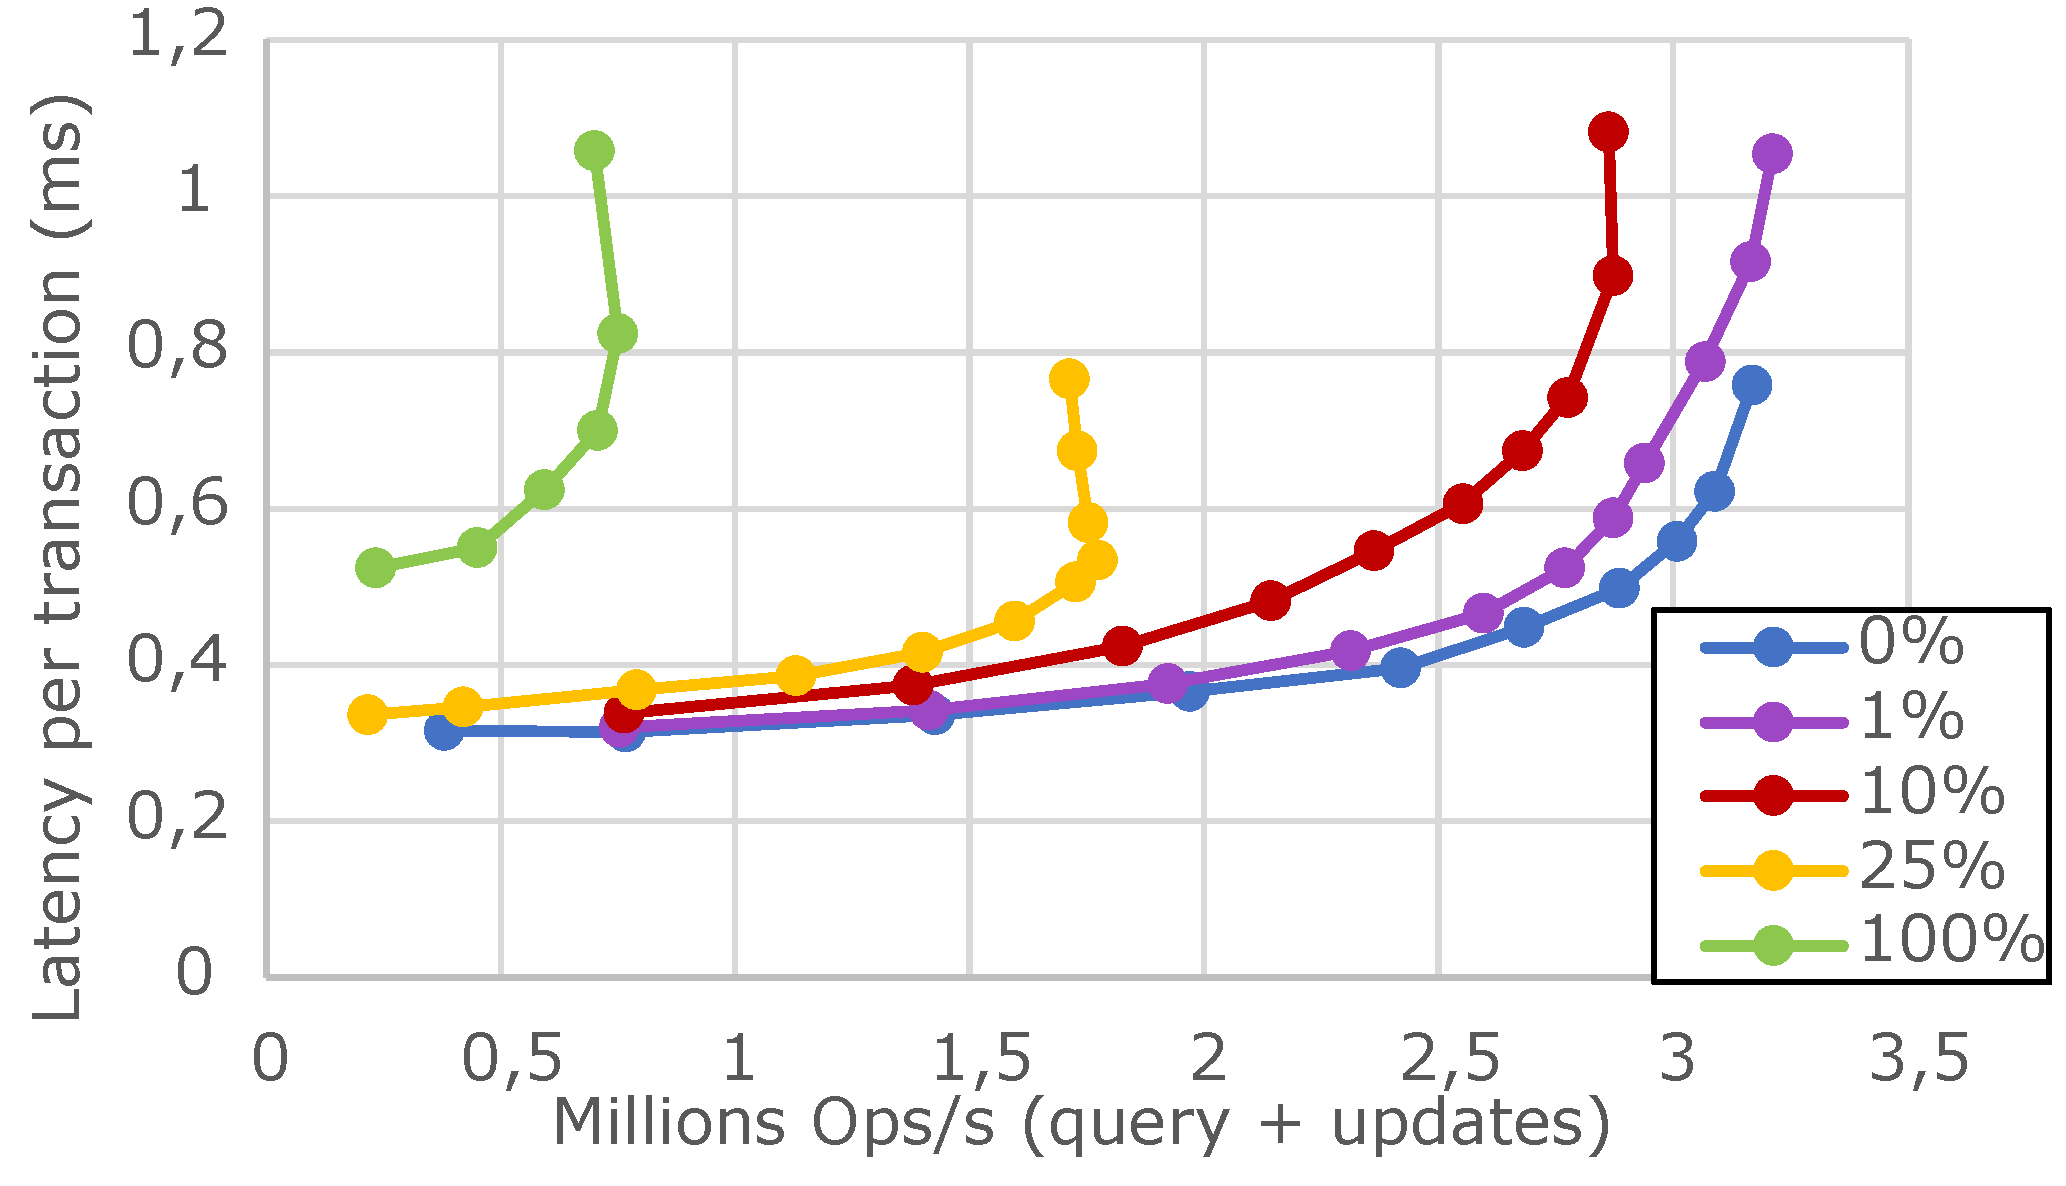
\includegraphics[width=.75\linewidth]{updRate_global_cut}
%	\caption{PotionDB's performance with varying update rate.}
%	\label{fig:(new)update_rates}
%\end{figure}
%
%\begin{figure}[h]
%	\centering
%	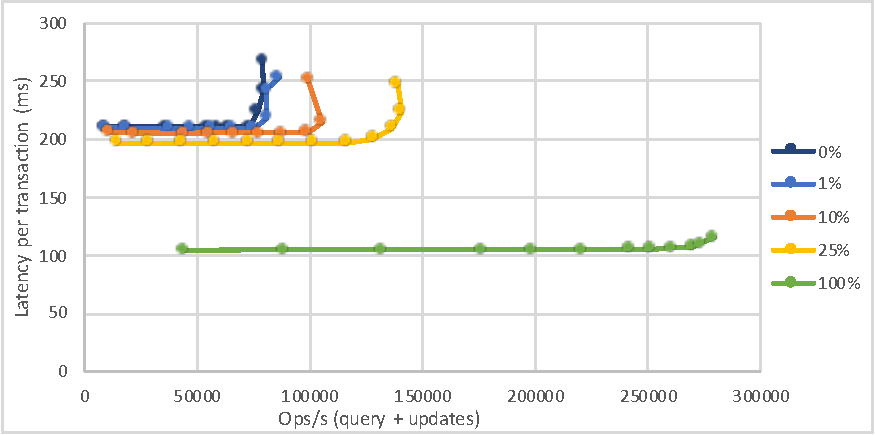
\includegraphics[width=.7\linewidth]{updRate_tc_cut}
%	\caption{Local PotionDB's performance with varying update rate}
%	\label{fig:(new)update_rates_tc}
%\end{figure}
%
%%Graph local: Low max throughput and high latency. Increasing the update ratio decreases latency slightly and increases max throughput con
%
%\begin{itemize}
%	\item Explain what is an update in TPC-H; explain how we do not count with view updates for the throughput;
%	\item Explain why PotionDB is unaffected by the added latency; explain why PotionDB's throughput decreases so heavily. Mention that a lot of the operations are not counted, as there are many view updates.
%	\item Explain why Local PotionDB is affected by the added latency. Explain why Local PotionDB's throughput increases with the higher update ratio and why latency decreases (reason: updates have lower latency than queries because only a subset of the servers need to be contacted, instead of all, so often the highest latency connection can be avoided. Furthermore, updates have more operations per transaction than queries, i.e., more operations per round trip.)
%\end{itemize}

\subsection{Performance under low latency among servers}
\label{subsec:potiondbSingleDC}

We now study whether keeping global views in all replicas is still interesting with low latency among replicas,
as in availability zones in a cloud region, using the extreme case with no added latency among servers running in the same DC.


\begin{figure}
	\centering
	\begin{subfigure}{.485\linewidth}
		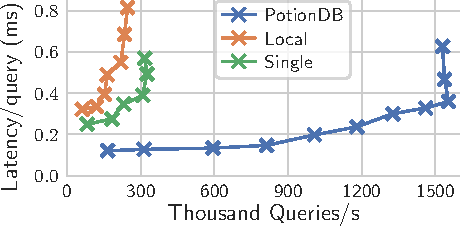
\includegraphics[width=1\linewidth]{singleQuery/all_queries_noTC}
	\vspace{-15pt}
		\caption{All queries}
		\label{fig:all_queries_noTC}
	\end{subfigure}%
	\hspace*{0.4em}
	\begin{subfigure}{.485\linewidth}
		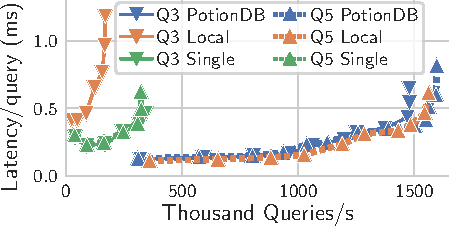
\includegraphics[width=1\linewidth]{singleQuery/q3_q5_noLatency}
	\vspace{-15pt}
			\caption{Single type of query}
		\label{fig:q3_q5_noTC}
	\end{subfigure}%
	\vspace{-10pt}
	\caption{Query performance in single DC.}
	\label{fig:global_local_single_noTC}
	\vspace{-15pt}
\end{figure}


Figure \ref{fig:global_local_single_noTC} present the results for read-only workloads.
The results for \textit{PotionDB} are similar to the previous results - this is expected as all operations are local.
\textit{Local} and \emph{Single} have much lower latency and higher throughput when compared with the
geo-distributed setting. This is expected due to the low latency for contacting other replicas now.
% - a intra-DC only the latency of contacting a node in the same data center. 
The maximum throughput is still much lower than that
of \textit{PotionDB}, as the need to contact multiple servers for replying to a query induces 
an higher load in the servers. 

For the results with a single query - Figure \ref{fig:q3_q5_noTC} - the trend is similar to 
the results for the geo-replicated setting, but with an increased throughput and lower latency
for \textit{Local} and \textit{Single}, due to the low latency for contacting other replicas. 


\begin{figure}
	\centering
	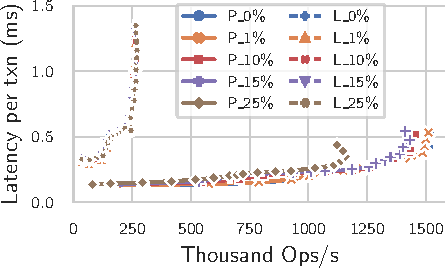
\includegraphics[width=0.62\linewidth]{singleQuery/upd_rate_noTC_global_vs_local}
	\vspace{-10pt}
	\caption{Performance with updates and no added latency.}
	\label{fig:update_rates_global_vs_local_noTC}
	\vspace{-12pt}
\end{figure}

%TODO: Would be really nice if I could trim this one further
The results for workloads with updates, presented in Figure~\ref{fig:update_rates_global_vs_local_noTC}, 
shows similar trends - PotionDB maintains a significantly better performance than alternative
approaches, which improve throughput and lower latency.  


%similar trends occur with updates, similar conclusions can be taken - Figure \ref{fig:update_rates_global_vs_local_noTC} showcases PotionDB's and Local PotionDB's throughputs for multiple update rates.
%PotionDB's throughput is the same as previously in Figure \ref{fig:update_rates_global_single_tc}.
%%PotionDB is the same as previously observed in Figure \ref{fig:update_rates_global_single_tc}. %, given latency between servers does not affect PotionDB's performance.
%Local PotionDB's throughput only reaches $\sim$250k ops/s for all update rates.
%%For Local PotionDB, the throughput is lower than PotionDB's in all cases, staying at around 250k ops/s for all update rates.
%The stability of Local PotionDB's throughput across different update rates is threefold:
%%Local PotionDB's stable throughput across different update rates is threefold:
%\begin{enumerate*}[label=(\roman*)]
%	\item multiple updates per transaction;%, unlike queries which are one per transaction;
%	\item orders' locality, thus many update transactions are local;
%	%\item orders' locality implies half of update transactions are fully local and most others involve only a subset of servers;
%	\item view updates are not replicated as views are local, which slightly reduces server load. %"do not need to be replicated" instead of "are not replicated"
%	%\item view updates do not need to be replicated unlike in PotionDB as views are local, thus slightly reducing server load.
%	%\item orders' locality implies that half of update transactions can be executed fully locally, with most others only requiring a subset of servers, unlike global queries which require all servers;
%	%\item since views are local, view updates do not need to be replicated and applied in other servers, thus slightly reducing server load.
%\end{enumerate*} %This still has some overlap with the previous section
%Update scenarios favour Local PotionDB, yet its performance is far from PotionDB's.
%%Even though scenarios with updates are favourable for Local PotionDB, it still does not match PotionDB's performance even with an high update ratio.
%Finally, Single PotionDB's thoughput is similar to what was observed in Figure \ref{fig:update_rates_global_single_tc} (and thus lower than PotionDB's), but with lower latencies ranging from 0.24ms to 0.6ms.
%%Finally, Single PotionDB achieves a throughput similar to what was observed previously in Figure \ref{fig:update_rates_single_tc}, but with smaller latencies, ranging from 0.2ms to 0.6ms.
%%Its throughput is, thus, still always lower than PotionDB's.

To conclude, PotionDB's global views provide query throughput and latency unmatched by alternative 
\textit{Local} and \emph{Single} approaches in every tested scenario.
We note, however,  that there are additional resources used for maintaining views in all replicas and this
should be considered when deciding whether to adopt this approach or not in a single data center.


%\subsection{Types of views (or maybe, Views type benchmarking?}
\subsection{Performance of different types of views}
\label{subsec:microbenchmarks}

%Next, we explore how different views behave and scale for different configurations. 
In this section we study the performance of the underlying NuCRDTs supporting different types of 
views: simple limits (Top-K), limits over aggregations (Top-K counter), sum/count (Counter) and average (Average) aggregations.
These experiments use micro-benchmarks, where clients access single NuCRDTs directly and could
also be used to infer the performance of applications with simple view requirements - for example, in a social
network, a materialized list of recent posts can be implemented using a Top-K and a list with the posts with more likes 
can be implemented as a Top-K counter.

We run the experiments with the same configuration - 10 machines
divided in 5 groups, with one machine for the server and another for running clients, with no
additional latency added to communications.  
%We run the experiments with the same configuration as the previous experiments - 10 machines
%divided in 5 groups, with one machine for the server and another for running clients, with no
%additional latency added to communications.  
In each experiment, we have 20 CRDTs.
Top K and Top K Counter CRDTs are initialized with 10K elements. 
Clients execute transactions consisting in read and updates operations, with each operation 
executed in a CRDT selected randomly using an uniform distribution. For Top K, updates
are insert and remove of a random elements; for top K counter, updates are increment 
and decrement to a random element.
Unless stated otherwise, each transaction consists in a batch of 5 operations.


\begin{figure}
	\centering
	\begin{subfigure}{.471\linewidth}
		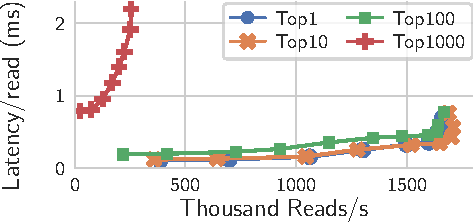
\includegraphics[width=1\linewidth]{singleQuery/bench_top_size_0_upd}
	\vspace*{-10pt}
			\caption{1 read per txn.}
		\label{fig:topSize_single}
	\end{subfigure}%
	\hspace*{0.2em}
	\begin{subfigure}{.509\linewidth}
		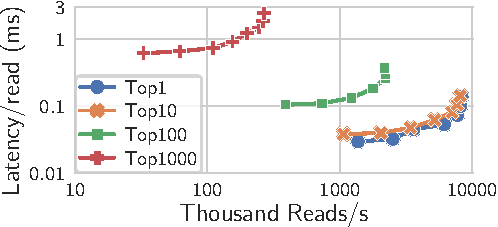
\includegraphics[width=1\linewidth]{singleQuery/bench_top_size_0_upd_5b}
	\vspace*{-10pt}
		\caption{5 reads per txn (log scale).}
		\label{fig:topSize_batch}
	\end{subfigure}%
	\vspace*{-10pt}
	\caption{TopK query performance for multiple top sizes.}
	\label{fig:topSize}
	\vspace*{-10pt} %TODO: Increase this once we can pull higher the text
\end{figure}

%TODO: Maybe not focus so much on serialization/deserialization: it may not be easy to justify/not the real cause

\noindent
\textbf{Scalability of Top-K and Top-K Counter.} %\hspace{0em}
We start by analysing the performance benefit of clients batching operations. %Andre: added as reviewer 370B asked "where  is this batching happening" 
%We start by studying the impact of batch size in the number of operations executed. 
Figures \ref{fig:topSize_single} and \ref{fig:topSize_batch} present the results for a read-only workload accessing
top-K objects, where transactions include, respectively, 1 read operation and 5 read operations.
The results show that, for small tops - Top-1 and Top-10, the number of operations executed increases almost
linearly with the number of reads in the transaction. In this case, the fixed overhead of setting 
up a transaction and sending messages dominates the load. 
For larger tops, the number of operations executed increases less. In this case, the amount of data 
transmitted becomes increasingly more relevant in the performance of the system.
We expect that with tops larger than 1000, the number of operations performed when using batches will 
tend to be similar to that of when performing reads independently.


%The results show that Top1, Top10 and Top100 all perform similarly with 1 read per txn, as communication overhead 
%for small messages (latency, metadata, serialization and deserialization of protobufs) and high number of clients 
%dominate over costs of data transfer and query execution time.
%
%
%
%Grouping reads reduces the aforementioned overhead - with 5 reads per transaction, throughput from Top1 to Top10 drops very slightly ($\sim$2\%), with a much bigger drop for Top10 to Top100 ($\sim$73\%) and Top100 to Top1000 ($\sim$88\%).
%In the latter two cases the amount of data transferred for the replies is the dominating factor, thus making better usage of the network's bandwidth.
%We expect that after 1000, increasing K linearly will decrease throughput linearly as well.
%%by the same factor.


\begin{figure}
	\centering
	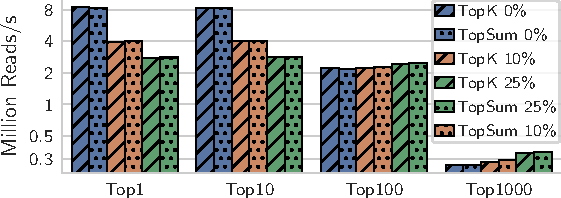
\includegraphics[width=0.76\linewidth]{singleQuery/topk_vs_topsum_5b}
	%\caption{TopK vs TopSum for multiple Top sizes and update ratios}
	\vspace*{-0.6em}
	\caption{Performance of Top K vs Top K Counter (TopCnt).}
	\label{fig:topKVSTopSum}
	\vspace*{-0.75em}
\end{figure}

We now compare how Top K and Top K Counter behave for different values of K, with different update
ratios. For updates, we use an add/remove ratio of 90\%/10\%, as it is unusual for an element to be removed
from being considered for a top~\cite{Cabrita17Nonuniform} (note that a top K object keeps information about 
all elements in a partitioned way, with only the top K element being replicated in all replicas). 
Figure \ref{fig:topKVSTopSum} shows that both TopK and Top K Counter maximum throughput is similar, 
showing that the mechanism used for deciding when it is necessary to propagate updates for Top K Counters 
performs well. When considering different update ratios, for small tops, the throughput decreases with an increasing 
ratio of updates, as processing updates is more complex than reads. For larger tops, the throughput with
a larger ratio of updates increases as the overhead of returning the larger tops to clients becomes the dominating 
factor of the performance of the system.


%Thus, we now focus on update scalability.
%%The results with updates are somewhat different to query-only.
%The size of an update is independent of the top's size - thus, as the amount of updates increase and reads decrease, throughput increases considerably for Top1000 and slightly for Top100.
%%Although adding/removing elements gets more expensive as K increases (higher chance for the actual top to be modified), this is offset by the cost of transferring all K elements over the network as a read reply. 
%%TODO: Would be nice to re-add the one above.
%Conversely, Top1 and Top10's throughput decreases as the update ratio goes up, %as commits for updates lock shards, thus reducing read parallelism.
%as commits for updates reduce read parallelism.


\nuno{Interessante, mas sem resultado a comprovar isto pareceria completa especulação.}
%TODO: I would love to leave this here but I feel like I should omit it. Or maybe make it even shorter
\nuno{As a final note, without batching the throughput with updates keeps up better with the query-only scenario.
For instance, Top 10 with 0\% to 25\% updates goes from 8.19M to 2.23M (-72.8\%) and 1.7M to 1.12M (-34.1\%) ops/s for, respectively, 5 and 1 operations per transaction.
Multi-update transactions lock multiple shards instead of just one, so they reduce available parallelism more than single updates do.
}
%The higher drop is because multi-update transactions lock multiple shards instead of only one, thus reducing parallelism for commits and reads.
%As a final note, without batching of neither reads or updates the throughput with updates keeps up better with the query-only scenario.
%Namely, for Top10 with 0\%, 10\% and 25\% updates, with a single operation per transaction, Top10 achieves 1.7M, 1.27M (-25.3\%) and 1.12M (-34.1\%) ops/s, while with 5 operations per transaction it achieves 8.19M, 4M (-51.1\%) and 2.23M (-72.8\%) ops/s.
%This bigger difference is because update transactions with multiple updates can not commit as much in parallel as when only with a single update, as the former has to lock multiple shards instead of just one.


\begin{figure}
	\centering
	\begin{subfigure}{.325\linewidth}
		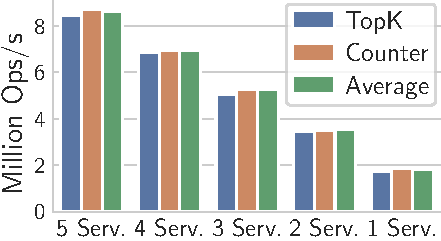
\includegraphics[width=1\linewidth]{singleQuery/n_servers_0_upd_5b}
	\vspace*{-10pt}
		\caption{Query-only}
		\label{fig:crdts_0_upd}
	\end{subfigure}%
	\begin{subfigure}{.325\linewidth}
		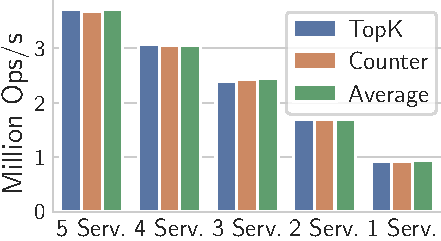
\includegraphics[width=1\linewidth]{singleQuery/n_servers_0_1_upd_5b}
	\vspace*{-10pt}
		\caption{10\% updates.}
		\label{fig:crdts_10_upd}
	\end{subfigure}%
	\begin{subfigure}{.34\linewidth}
	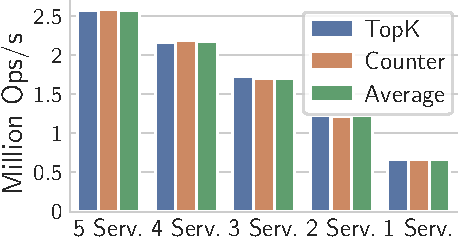
\includegraphics[width=1\linewidth]{singleQuery/n_servers_0_25_upd_5b}
	\vspace*{-10pt}
	\caption{25\% updates.}
	\label{fig:crdts_25-upd}
	\end{subfigure}%
	\vspace*{-10pt}
	\caption{Performance of NuCRDT.}
	\label{fig:crdts:perf}
	\vspace*{-15pt}
\end{figure}

\noindent
\textbf{Impact of the number of replicas.}
We now evaluate how NuCRDTs that support views scale with the number of replicas. 
Figure \ref{fig:crdts:perf} shows the throughput of NuCRDTs with different numbers of replicas
(for top K,  we used K = 10). 
%Results are presented in Figure~\ref{fig:crdts:perf}. 
We observe that, 
for each configuration the throughput is similar.  This shows that the internal implementation of
the CRDT has little impact in the overall throughput of the system, even if internally NuCRDTs are
considerably different.

For read-only workloads, the throughput with 5 replicas is almost 5$\times$
the throughput with a single replica - this is expected as operations execute locally in each replica. 
For workloads with updates, the throughput for 25\% updates in a system with 5 replicas is
close to 4$\times$ the
throughput of a system with a single replica. This lower scale-out was expected, as updates need to execute in all replicas,
imposing some additional load in all servers.


%%PotionDB scales well both with and without updates.
%With queries only, scalability is near linear on the number of replicas - e.g., Average with 1 server (1S) has 21.2\% of 5S' throughput of 8.62M ops/s.
%With updates, max throughput is smaller and scalability is less linear - e.g., for 25\% updates, Average with 1S has 25.9\% of 5S' throughput of 2.57M ops/s.
%PotionDB's scalability even with updates is solid given each replica applies around 4 times more updates with 5S than with 1S.
%PotionDB's replication mechanism groups remote transactions together, allowing for efficient execution.
%%When executing only queries, throughput scalability is close to linear as reads are locally served - e.g., Average goes from 8.62M ops/s with 5 servers (5S) to 6.92M ops/s with 4S (-19.7\%) and to 1.83M ops/s with 1S (-78.8\%).
%%With updates, max throughput is lower and scales down less linearly, as updates must be propagated and executed in all replicas.
%%E.g., Average with 25\% update rate goes from 2.57M ops/s with 5S to 2.17M ops/s with 4S (-15.6\%) and to 0.665M ops/s with 1S (-74.1\%).
%%However, despite each replica applying around 4 times more updates with 5S than with 1S, the scalability loss is modest.
%%%However, despite the number of updates effectively applied in each server being around 4 times higher with 5 replicas than with 1 replica, the loss on scalability is modest.
%%This is because PotionDB's replication mechanism groups transactions together, allowing for efficient execution.
%%This is because PotionDB's replication mechanism groups updates from different transactions, allowing them to be executed efficiently. %TODO: Maybe add reference to Replication section if I mention this there.

%\subsection{Scalability of number of views}
%
%%IMPORTANT NOTE: I believe with batching of queries, the throughput would decrease as the number of views increase. But for now, the major cost is on communication and locking (lock for TM's clock) in TM.
%
%Next, we experiment how the number of views affects PotionDB's performance.
%As keeping materialized views up-to-date imposes extra updates when a new order is added, it is expected for PotionDB's performance to worsen with a higher number of supported views. %Maybe this phrase is not necessary.
%
%Figure \ref{fig:queryScaleUpds} showcases PotionDB's and Local PotionDB's performance, with different update rates and number of supported TPC-H queries.
%In a query-only scenario (P 0\% and L 0\%), there is no observable impact, as well as with P 1\% and P 10\%. %And I suppose (for 0% upd rate) this makes sense for as long as there's enough RAM available.
%Even with a high update ratio (P 25\%), PotionDB still achieves high throughput.
%It may seem odd that with 3 types of queries, the throughput of P 25\% is lower than with more queries - this happens as with a lower variety of queries, they have to wait more often for updates to finish. %Not sure if this is clear - my theory is that with few types of queries, when a query arrives it's very likely its view is being updated. If we have many different queries, it's possible some queries arrive for views that already finished updating. Remember that in this experiments we're using Read Commited consistency. 
%%Even with a modest update ratio (P 25\%), PotionDB still maintains a high throughput. 
%%I think one of the queries I picked for 9 queries is costly for updating.
%Meanwhile, in Local PotionDB, throughput decreases slightly as the number of views increases.
%This happens as orders whose items come from multiple regions imply updates to views spread across servers, leading to higher synchronization costs. %My excuse is that with Local, when adding a new order, many view updates need to be forwarded from one server to the other, wasting precious bandwith on every txn.
%
%%\begin{figure*}
%%	\centering
%%	\begin{subfigure}{.19\linewidth}
%%		%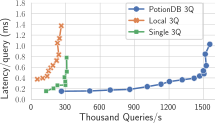
\includegraphics[width=1\linewidth]{queryScale/queries_scale_3Q}
%%		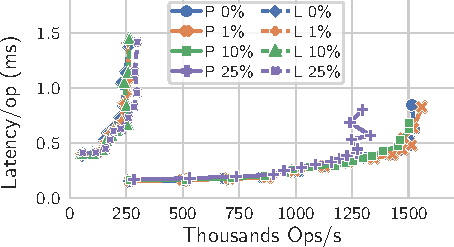
\includegraphics[width=1\linewidth]{queryScale/3Ops}
%%		\caption{Queries: 3, 11, 14.\\\hspace{\textwidth}}
%%		\label{fig:3Q}
%%		%\vspace*{0.7em}
%%	\end{subfigure}%
%%	\hspace*{0.3em}
%%	\begin{subfigure}{.19\linewidth}
%%		%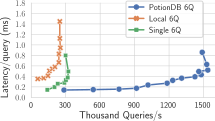
\includegraphics[width=1\linewidth]{queryScale/queries_scale_6Q}
%%		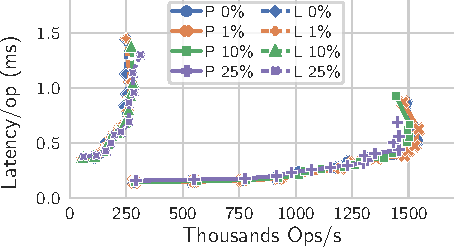
\includegraphics[width=1\linewidth]{queryScale/6Ops}
%%		\caption{Queries:\\\hspace{\textwidth} 3, 5, 11, 14, 15, 18.}
%%		\label{fig:6Q}
%%		%\vspace*{0.7em}
%%	\end{subfigure}%
%%	\hspace*{0.3em}
%%	\begin{subfigure}{.19\linewidth}
%%		%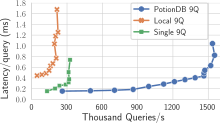
\includegraphics[width=1\linewidth]{queryScale/queries_scale_9Q}
%%		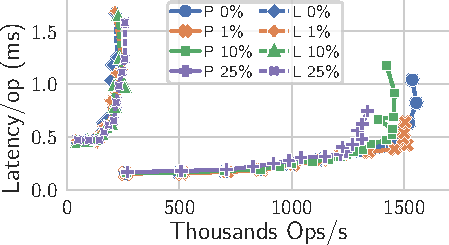
\includegraphics[width=1\linewidth]{queryScale/9Ops}
%%		\caption{Queries:\\\hspace{\textwidth} 2, 3, 5, 8, 11, 13-15, 18.}
%%		\label{fig:9Q}
%%		%\vspace*{0.7em}
%%	\end{subfigure}%
%%	\hspace*{0.3em}
%%	\begin{subfigure}{.19\linewidth}
%%		%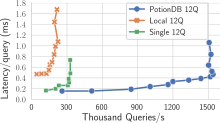
\includegraphics[width=1\linewidth]{queryScale/queries_scale_12Q}
%%		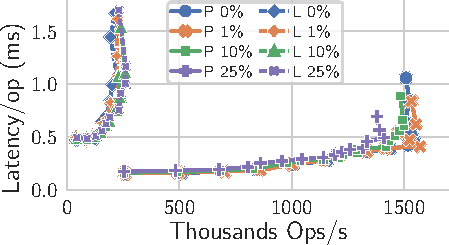
\includegraphics[width=1\linewidth]{queryScale/12Ops}
%%		\caption{Queries:\\\hspace{\textwidth} 2, 3, 5-8, 11, 13-15, 17, 18.}
%%		\label{fig:12Q}
%%		%\vspace*{0.7em}
%%	\end{subfigure}%
%%	\hspace*{0.3em}
%%	\begin{subfigure}{.19\linewidth}
%%		%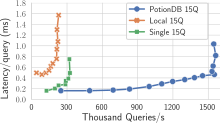
\includegraphics[width=1\linewidth]{queryScale/queries_scale_15Q}
%%		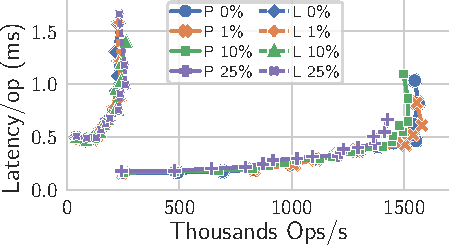
\includegraphics[width=1\linewidth]{queryScale/15Ops}
%%		\caption{Queries:\\\hspace{\textwidth} 2-8, 11-15, 17, 18, 21.}
%%		\label{fig:15Q}
%%		%\vspace*{0.7em}
%%	\end{subfigure}%
%%	\vspace*{-0.65em}
%%	\caption{PotionDB and Local PotionDB  performance with multiple update rates and an increasing number of views.}
%%	\label{fig:queryScaleUpds}
%%	\vspace*{-0.2em}
%%\end{figure*}
%
%\subsection{Scalability of number of views}

%IMPORTANT NOTE: I believe with batching of queries, the throughput would decrease as the number of views increase. But for now, the major cost is on communication and locking (lock for TM's clock) in TM.

%Keeping materialized views up-to-date requires updating all affected views when a new order is added. 
%We now evaluate how the number of views impacts PotionDB's performance.


%Next, we experiment how the number of views affects PotionDB's performance.
%As keeping materialized views up-to-date imposes extra updates when a new order is added, it is expected for PotionDB's performance to worsen with a higher number of supported views. %Maybe this phrase is not necessary.

%Figure \ref{fig:queryScaleUpds} showcases \textit{PotionDB}'s and \textit{Local}'s performance, with different update rates and number of supported TPC-H queries.
%In a query-only scenario (P 0\% and L 0\%), there is no observable impact, as well as with P 1\% and P 10\%. %And I suppose (for 0% upd rate) this makes sense for as long as there's enough RAM available.
%Even with a high update ratio (P 25\%), PotionDB still achieves high throughput.
%It may seem odd that with 3 types of queries, the throughput of P 25\% is lower than with more queries - this happens as with a lower variety of queries, they have to wait more often for updates to finish. %Not sure if this is clear - my theory is that with few types of queries, when a query arrives it's very likely its view is being updated. If we have many different queries, it's possible some queries arrive for views that already finished updating. Remember that in this experiments we're using Read Commited consistency. 
%Even with a modest update ratio (P 25\%), PotionDB still maintains a high throughput. 
%I think one of the queries I picked for 9 queries is costly for updating.
%Meanwhile, in Local PotionDB, throughput decreases slightly as the number of views increases.
%This happens as orders whose items come from multiple regions imply updates to views spread across servers, leading to higher synchronization costs. %My excuse is that with Local, when adding a new order, many view updates need to be forwarded from one server to the other, wasting precious bandwith on every txn.

%\begin{figure*}
%	\centering
%	\begin{minipage}{.58\linewidth}
%		\centering
%	\begin{subfigure}{.32\linewidth}
%		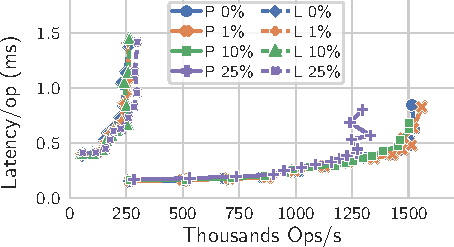
\includegraphics[width=1\linewidth]{queryScale/3Ops}
%		\caption{Queries: 3, 11, 14.\\\hspace{\textwidth}}
%		\label{fig:3Q}
%		%\vspace*{0.7em}
%	\end{subfigure}%
%	\hspace*{0.3em}
%	\begin{subfigure}{.32\linewidth}
%		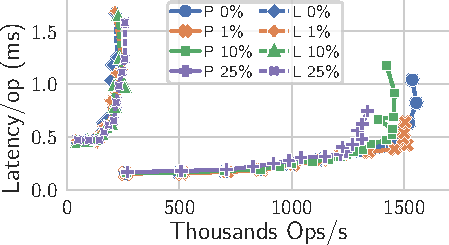
\includegraphics[width=1\linewidth]{queryScale/9Ops}
%		\caption{Queries:\\\hspace{\textwidth} 2, 3, 5, 8, 11, 13-15, 18.}
%		\label{fig:9Q}
%		%\vspace*{0.7em}
%	\end{subfigure}%
%	\hspace*{0.3em}
%	\begin{subfigure}{.32\linewidth}
%		%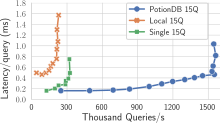
\includegraphics[width=1\linewidth]{queryScale/queries_scale_15Q}
%		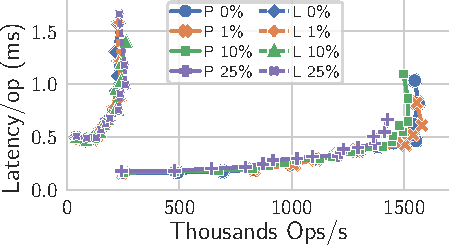
\includegraphics[width=1\linewidth]{queryScale/15Ops}
%		\caption{Queries:\\\hspace{\textwidth} 2-8, 11-15, 17, 18, 21.}
%		\label{fig:15Q}
%		%\vspace*{0.7em}
%	\end{subfigure}%
%	\vspace*{-0.65em}
%	\caption{PotionDB and \emph{Local}  performance with multiple update rates and an increasing number of views.}
%	\label{fig:queryScaleUpds}
%	\vspace*{-0.2em}
%	\end{minipage}%
%	\hspace*{0.05\linewidth}
%	\begin{minipage}{.34\linewidth}
%		\centering
%		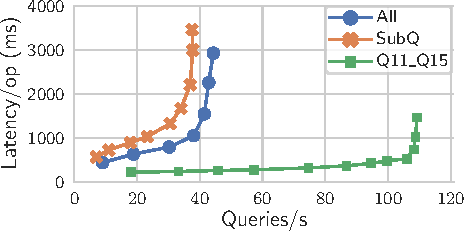
\includegraphics[width=0.8\linewidth]{postgres/postgresNoView}
%		%\vspace*{-0.65em}
%		\caption{PostgreSQL query performance with indexes instead of materialized views. Notice that the x axis is in the scale of units.}
%		\label{fig:postgresNoViews}
%	\end{minipage}
%\end{figure*}

\subsection{Comparison with PostgreSQL}\label{sec:eval:postgrs}

%For the sake of completion, 

In this section we compare PotionDB with PostgreSQL \cite{PostgreSQL}.  

\noindent
\textbf{Incremental view maintenance.} %\hspace{0em}
In these experiments, we used pg\_ivm - PostgreSQL's incremental view maintenance extension \cite{ivm}. 
As pg\_ivm  cannot be used with PostgreSQL's Logical Replication \cite{PostgreSQLLogical}, it is not possible to configure PostgreSQL with partial replicas.
Thus, our configuration with PostgreSQL has a single server, with all operations being propagated to this server - this is akin to \textit{Single} configuration. 
For speeding up PostgeSQL, we use asynchronous commit with read committed and a 64GB RAM disk for storage. 

%We now compare PotionDB with PostgreSQL \cite{PostgreSQL}, a well known, robust, open-source RDBMS.
%We deploy a single PostgreSQL instance on a 64GB RAM disk. %I also adjusted other settings to boost Postgre's performance, like increasing max number of connections, work memory, etc.
%PostgreSQL does not natively support incremental view maintenance, thus the pg\_ivm extension \cite{ivm} is used.
%Pg\_ivm has some limitations, namely it prevents the usage of PostgreSQL's Logical Replication \cite{ivm, PostgreSQLLogical}, hence the usage of a single server.
%The subset of SQL usable for specifying views with pg\_ivm is also limited, namely it is not possible to compose views, compose aggregations, do \emph{order by} among others, which limits the expressivity of views and negatively impacts query performance. %Not sure if I should mention this here. For our subset of queries, Q15 is the one affected by these limitations.
%For fairness, we focus on comparing PostgreSQL with Single PotionDB.
%Clients are assumed to be running in the same data center as the server(s). %TODO: Justification/motivation for this? I just wanted to leave clear we did not add any latency.

\begin{figure*}[t]
	\centering
	\begin{minipage}{.57\linewidth}
		\begin{subfigure}{.482\linewidth}
			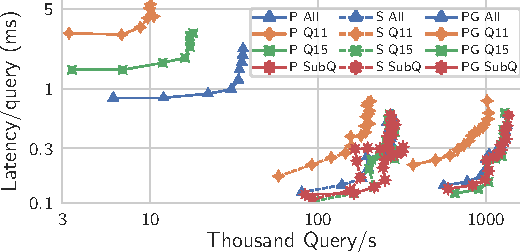
\includegraphics[width=1\linewidth]{postgres/postgresQueryOnly}
	\vspace{-10pt}
			\caption{Query-only.}
			\label{fig:postgres_query}
		\end{subfigure}%
		\hspace*{0.4em}
		\begin{subfigure}{.483\linewidth}
			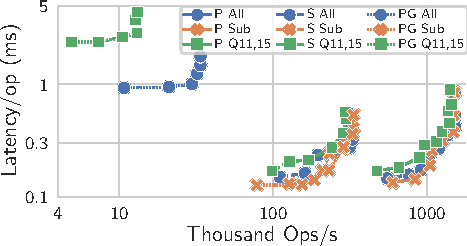
\includegraphics[width=1\linewidth]{postgres/postgresUpdateOnlyOps}
	\vspace{-10pt}
			\caption{1 update, multiple query clients.}
			\label{fig:postgres_update}
		\end{subfigure}%
	\vspace{-10pt}
		\caption{Comparison with PostgreSQL - All represents all selected queries; Sub consists of Q3, Q5, Q14 and Q18.}
%	\caption{Postgres vs PotionDB. P, S and PG stand for, respectively, PotionDB, \emph{Single} and Postgres. All represents all selected queries;  Sub consists of Q3, Q5, Q14 and Q18.}
		%All represents all selected queries, SubQ consists of Q3, Q5, Q14 and Q18, SubU consists of Q11, Q14 and Q18.}
		\label{fig:postgres}
	\vspace*{-0.2em}
	\end{minipage}%
	\hspace*{0.07\linewidth}
	\begin{minipage}{.36\linewidth}
		\centering
		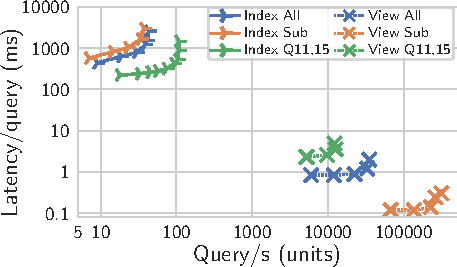
\includegraphics[width=0.85\linewidth]{postgres/postgresViewVsIndex}
		%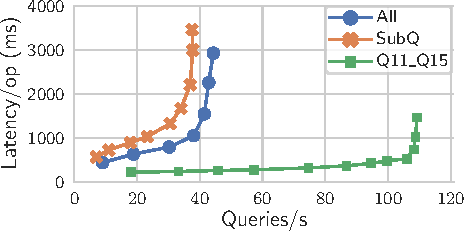
\includegraphics[width=0.85\linewidth]{postgres/postgresNoView}
		\vspace*{-10pt}
		\caption{PostgreSQL query-only performance with indexes.}
		%\caption{PostgreSQL query performance with indexes instead of materialized views. Notice that the x axis is in the scale of units.}
		\label{fig:postgresNoViews}
	\vspace{-10pt}
	\end{minipage}
	\vspace{-10pt}
\end{figure*}

%\begin{figure}
%	\centering
%	\begin{subfigure}{.482\linewidth}
%		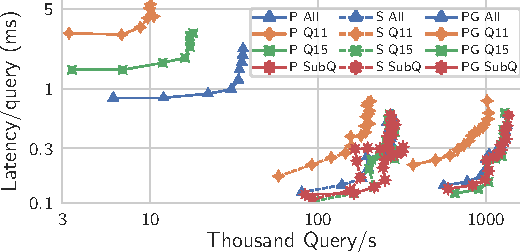
\includegraphics[width=1\linewidth]{postgres/postgresQueryOnly}
%		\caption{Query-only  throughput.}
%		\label{fig:postgres_query}
%		\vspace*{0.7em}
%	\end{subfigure}%
%	\hspace*{0.3em}
%	\begin{subfigure}{.483\linewidth}
%		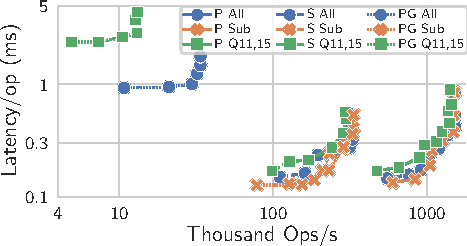
\includegraphics[width=1\linewidth]{postgres/postgresUpdateOnlyOps}
%		\caption{Throughput with multiple query clients and 1 update client.}
%		\label{fig:postgres_update}
%	\end{subfigure}%
%	\vspace*{-0.65em}
%	\caption{Postgres vs PotionDB. P, S and PG stand for, respectively, PotionDB, \emph{Single} and Postgres. All represents all selected queries;  Sub consists of Q3, Q5, Q14 and Q18.}
%		%All represents all selected queries, SubQ consists of Q3, Q5, Q14 and Q18, SubU consists of Q11, Q14 and Q18.}
%	\label{fig:postgres}
%	\vspace*{-0.2em}
%\end{figure}

%\begin{table}
%	\begin{tabular}{l | a | b | a | b}
%		\hline
%		\rowcolor{LightCyan}
%		\mc{}{}  & \mc{1}{x} & \mc{1}{y} & \mc{1}{w} & \mc{1}{z} \\
%		\hline
%		PotionDB & a & b & c & d \\
%		 & a & b & c & d \\
%		All & a & b & c & d \\
%		SubQ & a & b & c & d
%		 \hline
%	\end{tabular}
%\end{table}

Figure \ref{fig:postgres_query} shows that
both \textit{Single} and \textit{PotionDB} outperform \textit{PostgreSQL} (PG) for our read-only workload.
This is due to two queries - Q11 and Q15.
The other queries (Q3, Q5, Q14 and Q18) are well supported by PostgreSQL, with a performance similar to \textit{Single}, 
but far from \textit{PotionDB}. 
This shows that having replicated views over geo-partitioned data, as in PotionDB, is crucial to provide good performance.

Q15 is not efficient because pg\_ivm does not support \emph{order by} and aggregations of aggregations in views, requiring 
an extra computation when executing the query. Q11 is inefficient as it returns a large number of rows, which
turns out to be slower in PostgreSQL when compared with PotionDB.

%Figure \ref{fig:postgres_query} presents query-only performance.
%Both \textit{Single} and \textit{PotionDB} outperform considerably \textit{PostgreSQL} (PG) when executing all selected queries.
%This is mostly due to two of the selected queries - Q11 and Q15.
%The other queries (Q3, Q5, Q14 and Q18) are well supported by PostgreSQL, even slightly outperforming \emph{Single}, 
%but far from \emph{PotionDB}'s throughput.
%
%Q15 is not efficiently supported in PostgreSQL as pg\_ivm does not support both \emph{order by} nor aggregations of aggregations, thus to 
%answer this query extra computation is required and multiple rows are scanned. %It needs to calculate a "max" manually.
%On the other hand, Q11 is efficiently supported but returns more data than other queries do - 100 rows, instead of 10 or less.
%Thus, Q11 has reduced performance in both Single, PotionDB and PostgresSQL compared to other, simpler, queries. 
%However the max throughput reduction is much higher in PostgresSQL (96.8\%) than Single (28.5\%) or PotionDB (25.5\%). %Maybe with raw numbers the difference looks more significant? PostgresSQL: 320k -> 10k query/s. Single. 288k -> 206k. PotionDB: 1371k -> 1044k.

Figure \ref{fig:postgres_update} shows performance in a workload with queries and updates - results are similar to
the read-only workload. 
However, unlike the results presented in previous sections, these results were obtained having a single client executing
updates - in PostgreSQL, when there are concurrent update transactions in a database with multiple views (with incremental view maintenance), 
latency becomes very high and can reach a few seconds, which would lead to low performance if all clients performed updates. 
We note that is not the case in PotionDB, which can provide TCC with high throughput in workloads with up to 25\% of updates.



%Figure \ref{fig:postgres_update} showcases PostgresSQL's performance with both queries and updates.
%At a first glance, it looks similar to Figure \ref{fig:postgres_query}.
%However, this is due to two key limitations in this experiment:
%\begin{enumerate*}[label=(\roman*)]
%	\item \label{post1} updates insert only new orders - there is no removes;
%	\item \label{post2} a single client is dedicated to execute updates - all other clients are query-only.
%\end{enumerate*}
%These limitations are employed because in PostgresSQL, updates with incremental view maintenance are very slow, easily reaching latencies in order of seconds when deploying views for more than one query.
%Furthermore, we observed in other experiments (not included in this document) that if we allow several clients to execute updates, PostgresSQL's clients will spend a long time waiting for each other's updates to commit, thus achieving very low throughput.
%Finally, \emph{delete} updates are about 4 times slower than \emph{insert} updates.
%On a positive note, update execution in PostgresSQL does not have a visible impact in the throughput of query-only clients.
%We note that, as observed in Figures \ref{fig:upds_tc} and \ref{fig:update_rates_global_vs_local_noTC}, PotionDB supports modest update rates in all clients while still maintaining high throughput, as views updates are generated and applied quickly, unlike in PostgresSQL.


\noindent
\textbf{No views.} %\hspace{0em}
Cloud databases typically do not support views, and when they support views they do not support incremental view maintenance.
As a result, to access a consistent view of the data, it is necessary to run the query on the database when necessary.
Figure \ref{fig:postgresNoViews} shows that executing the read-only workload in PostgreSQL in 
a database without views is three orders of magnitude slower than using views.
This result is even more relevant as the PostgreSQL database included the indexes that help executing the
queries in the workload. 
It is known that executing TPC-H style queries is challenging \cite{dreseler20quantifying} and these 
results show that views can greatly improve performance. 
In this paper, we show how to circumvent these challenges and provide low latency and high throughput 
by keeping views that support TCC access.
From the results presented in this section we can also conclude that the results for \textit{Local} presented in previous sections can be seen
as an upper bound (and probably much better) of the performance that could be achieve in a geo-partitioned key-value store that 
does not maintain any views. 


%Finally, Figure \ref{fig:postgresNoViews} showcases PostgreSQL's query-only performance when using indexes to support the queries instead of views.
%When comparing to Figure \ref{fig:postgres_query}, it follows up that the selected TPC-H queries do not perform well even when using indexes optimized for these queries, as many rows still need to be scanned and joins calculated to answer the queries. %Q3 performs "OK" with indexes (1000Q/s), but that's still A LOT slower compared to with views (300000Q/s)
%Similar results is expected of other databases without views or some caching  mechanism.
%Without indexes, performance would degrade even further as full table scans would be necessary.

%The scenario is quite different when updates are considered.
%We consider a single update transaction to be a new order and its associated lineitems, however we count each order or item as one update.
%On average, a new order has 4 to 5 items.
%Figure \ref{fig:postgres_update} shows the update throughput when having a single client executing updates, and a varying number of query clients.
%In all cases, as the number of query clients increases, the update throughput diminishes. %I do not know what to say to justify this... basically the reason is that it's only 1 update client, so he will spend more time waiting for an "oportunity" to update among all ongoing queries. 
%Even with incremental view maintenance, view maintenance has a high impact on PostgreSQL's update throughput.
%This is observable as PostgreSQL has a reasonable throughput (up to 6.5k updates/s) when only Q11's views are deployed (Q11 does not require updating), however this throughput is quite lower with Q15, the cheapest view to update, and is unreasonable when views for more than one query are considered (e.g., Q11, Q14 and Q18) or all views are considered, going as low as 5 updates per second.
%On the other hand, both Single and PotionDB achieve higher update throughput in all situations, and have almost no observable impact of having multiple views to update. %Multiple update clients would be needed to saturate PotionDB, and it would lead to an even higher update throughput.
%TODO: Should I replace the Q11_Q14_Q18 line with only Q14_Q18? To show that even with only 2 queries, it's already bad. My reasoning for leaving Q11 in, is because Q11 is "for free" when it comes to updates.

%We note the following limitations on our update experiments.
%First, only a single update client is used, as even a small amount of update clients easily overwhelm Postgres when having views for more than one query. %I don't know how to mention this, but let's say having 5-10 update clients will easily make inserting a new order take 10s. If needed I can get more precise data on this.
%Secondly, order removal is around 4 times slower than inserting a new order, thus our experiments only include insertions.
%Both limitations favor PostgreSQL, as PotionDB easily supports a high update ratio (see Section~\ref{subsec:potiondbSingleDC}), and is not affected considerably by deletes vs insertions, except for very high update ratios. %NOTE: We do not have any graph in the paper to support the last statement.


%\newpage
\section{Related Work}
\label{sec:related_work}

%TODO: Veronica uses projection to improve queries, might be worth comparing to.

%Maybe should use only "Consistency" as the paragraph title?
Our work was influenced by works in several different areas.

\noindent
\textbf{Consistency in geo-replication.}
Database systems can be classified as being either strongly or weakly consistent.
Strong consistency systems \cite{spanner, slog, scatter, krikellas2010strongly, sconekv, lu2021epoch, hildred2023caerus, nguyen2023detock} provide a total order for transactions and are easier to work with.
However, coordination between data centers is required, leading to high latency in geo-distributed scenarios and compromised availability under network partitions \cite{cap}.
By relaxing consistency guarantees, weak consistency systems \cite{dynamo, couchDB, cassandra, chainreaction, cops, riak, eiger} can provide low latency, high throughput and better fault tolerance.
However, concurrency conflicts make those solutions harder to work with.
Casual consistency 
%is a weak consistency model that 
alleviates this problem, however anomalies can still be observed even with cross-object causality \cite{cops, burckhardt2013understanding, ferreira2023antipode}.
%Database systems can offer different levels of consistency, and are usually labelled as either strongly or weakly consistent.
%Strong consistency systems \cite{spanner, slog, scatter, krikellas2010strongly, redblue, megastore} are easier to work with as they provide a total order for their transactions.
%Strong consistency requires coordination between data centers, which leads to high latency in geo-distributed scenarios and, as implied by the CAP theorem \cite{cap}, network partitions compromise the system's availability.
%%However, the CAP theorem \cite{cap} implies that network partitions compromise availability.
%%However, the CAP theorem \cite{cap} implies that availability may be compromised in case of network partitions.
%%Furthermore, high latency is to be expected in geo-distributed scenarios as multiple data centers must be contacted for committing a transaction.
%By relaxing the provided consistency guarantees, weak consistency systems \cite{dynamo, couchDB, cassandra, chainreaction, cops, riak, eiger} can provide low latency, high throughput and better fault tolerance.
%However, concurrency conflicts make those solutions harder to work with.
%Causal consistency is a weak consistency model that alleviates this problem, however anomalies can still be observed even with cross-object causality \cite{cops, burckhardt2013understanding}.

\noindent
\textbf{Indexes and views.}
Both indexes and materialized views speed up query execution.
Indexes provide quick access to a table or an object using a non-primary key, often being used by queries requiring sorting or a given range of values.
Many systems implement indexes~\cite{dynamo, couchDB, cassandra, megastore} and there are several proposals on efficient usage and storage of indexes~\cite{lee2020asymmetric, lisa, bindex, slik, xiong2024civet, xu2024bp, hao2024bf}.
%slik
%On the other hand, 
%Conversely, 
Materialized views work as a cache for the result of a large query, avoiding expensive %data 
recalculations.
However, keeping views consistent and automatically updated is challenging \cite{oracleViews, chronocache, birds, budiu2023dbsp} and few systems implement them \cite{chronocache, marviq, estocada, couchDB, oracleViews, noria, clickhouse2024}, %even though they can speed up queries considerably.
despite their %considerable 
query speed-up potential and usefulness for analytic queries~\cite{analyticdb, hadad, sioulas2023real, clickhouse2024}.
%To the best of our knowledge, 
PotionDB is the first system to support materialized views of global data in a partially geo-replicated scenario.

%The paragraph below does not add anything new compared to the first paragraph. But maybe I could use it as inspiration to shorten the first paragraph
%Geo-distributed scenarios imply high latency when acessing far away data centers, which is required for strong consistency \cite{chronocache, slog, cops, eiger}. 
%Network partitions are also a concern, as they may render strongly consistent systems unavailable.
%Weak consistency can help avoid both problems but lacks the useful consistency guarantees provided by strong consistency.

%\andre{I still need to find citations for partial replication. Any suggestion/starting point is more than welcome}

\noindent
\textbf{Partial replication.}
Partial replication reduces storage costs and can potentially improve a system's performance, as less operations are applied on each server~\cite{sipre, optimisticPartial, coda, nguyen2023detock}, and is thus of interest for geo-distribution.
Careful data partitioning is essential to avoid clients having to contact far away servers, thus experiencing high latency~\cite{sipre, optimisticPartial, coda}.
However, queries over data sharded across data centers is challenging and slow, specially when providing a consistent snapshot.
PotionDB tackles this problem by providing views that summarize partially replicated data and directly answer such queries.

%\noindent
%\textbf{Partial Replication.}
%Partial replication reduces storage costs and can potentially improve a system's performance, e.g., due to less operations being applied on each server~\cite{sipre, optimisticPartial, coda}, and are thus of interest for geo-distribution.
%Data partitioning must be carefully done by considering where each object is relevant, as otherwise clients may need to access far away servers and thus experience high latency~\cite{sipre, optimisticPartial, coda}.
%However, one common problem with partial replication is that, sometimes, it is necessary to query data sharded among different data centers~\cite{sipre}.
%%Many systems provide partial replication \cite{???}.
%%However, a problem not often analyzed in these kind of systems is that some analytic queries may need to consult objects sharded between different data centers.
%Without views, this process can be slow, specially when trying to provide a consistent snapshot of the database.
%PotionDB tackles this problem by providing views that summarize partially replicated data and directly answer such queries.

%I made the CRDT paragraph shorter since we already talk about them in detail in other sections. Maybe should just remove it altogether?

%\noindent
%\textbf{CRDTs.} These replicated data types~ \cite{crdt} guarantee state convergence after applying the same set of operations.
%Thus they are often used in weakly consistent systems, e.g., Redis \cite{redisCRDT} and Riak \cite{riak}.
%Computational CRDTs \cite{computationalCrdt} and non-uniform CRDTs \cite{Cabrita17Nonuniform} are of particular interest for views in PotionDB, as the former summarizes data using aggregations, while the later minimizes the data stored and replicated between replicas while still ensuring queries are answered correctly.
%Maybe add example for Nu-CRDT? (e.g., a top-K CRDT does not need all entries to be replicated)
%\noindent
%\textbf{CRDTs.}
%Conflict-free Replicated Data Types, CRDTs \cite{crdt}, are replicated data types that guarantee state convergence as long as all updates are eventually delivered.
%Thus, they are often used in weakly consistent systems, e.g., Redis \cite{redisCRDT} and Riak \cite{riak}.
%Some types of CRDTs have been introduced that can help with representing views of data, namely computational CRDTs \cite{computationalCrdt} and non-uniform CRDTs \cite{Cabrita17Nonuniform}.
%The former computes some result over data (e.g., a sum), while the later focus on minimizing the information that needs to be replicated to correctly reply to queries (e.g.: a topK CRDT does not need all entries to be replicated).
%In PotionDB every object is a CRDT and, in particular, we leverage on both computational and non-uniform CRDTs to support our views.

\noindent
\textbf{Geo-distributed databases.}
Dynamo \cite{dynamo} and Cassandra \cite{cassandra} are eventually consistent databases.
Both provide indexes to speed up some queries but not materialized views, thus complex queries may need to access large amounts of objects.
CouchDB \cite{couchDB} provides both indexes and materialized views, however views can only refer to data in one partition.

ChronoCache \cite{chronocache} is a caching middleware for geo-replicated databases. 
% which focus on combining multiple queries into one request and caching query results.
While caching speeds up future requests, complex queries may still need to contact multiple servers and 
updates need to invalidade the cache or else clients read stale data.

%Caerus \cite{hildred2023caerus} implements a novel transaction algorithm for strongly consistent geo-dstributed databases.
%% which commits transactions with a single RTT.
%Data locality is leveraged on to reduce transaction latency.
%However, complex global queries still need to gather and process large amounts of data from multiple regions.
%%Furthermore, update transactions involving multiple regions still need to pay a full RTT.

%AnalyticDB \cite{analyticdb} focus on optimizing analytic queries. 
%It separates write and read paths to prevent complex queries from slowing down writes. 
%It also uses indexes to speed up queries. 
%However, complex queries still take hundreds of milliseconds to execute and may slow down  simpler queries.
%They do not make usage of views.

%This one is interesting as they leverage on partial replication and data locality to achieve low latency but nothing about views/query speedup.
%SLOG \cite{slog} provides ACID transactions in a geo-replicated scenario.
%By leveraging on partial replication and data locality (as in PotionDB), SLOG achieves low latency on transactions served by a single data center.
%However, queries regarding global data are slow and prone to network partitions.
%PotionDB's global views prevent both issues from happening.

%Not too relevant
%ESTOCADA \cite{estocada} is a system designed to work with polystores and focus on taking advantage of each database's stronger points and make extensive usage of the materialized views provided on each.

%Marviq \cite{marviq} tackles the specific situation of efficiently providing a visualization (e.g., scatterplot) of a large data set.
%Marvig leverages on materialized views to handle range queries and summarize large datasets.
%%While a very specific scenario, it showcases the need of summarizing large datasets.
%%Marviq leverages on materialized views for handling range queries.
%%While a more specific scenario than the one PotionDB aims for, it showcases similar challenges - large datasets that need to be sumarized and queried efficiently.
%%They make usage of materialized views to handle range queries on the datasets.

Magrino et. al. \cite{treaties} propose predictive treaties for efficient distributed computations. 
%The insight is that some computations can be expressed by treaties, and it is possible to anticipate a range of how a value might change over time.
Treaties use less data than PotionDB's materialized views but can give incorrect query replies as the ranges may be inaccurate.
Furthermore, it is unfeasible to predict changes for some data.
%Finally, given strong consistency is assumed, queries regarding global data will be slow when synchronization is required and prone to network partitions.

Noria \cite{noria} is a streaming data-flow system.
It leverages on views and partial data to provide fast query reply with reasonable memory usage.
While it features high throughput, it only offers eventual consistency, which complicates application development.
There is also concerns on the performance of queries when a view needs to be rebuilt and data is sharded.

ParCuR \cite{sioulas2023real} focus on optimizing analytic queries, recognizing the importance of low response times for analytic queries.
ParCuR combine two non-trivial techniques - subexpression materialization and work-sharing.
However, recurrent queries still require many repeated work, as materialized views are not directly deployed. 
Furthermore, neither geo or partial replication are considered, unlike in PotionDB.


%Should prob make a general comparison to MongoDB/Cassandra/Dynamo

%Comparison to specific solutions?

%Geo-replication, partial-replication

%CRDTs?

%\section{[OLD]Related Work}
%
%Both strongly and weakly consistent solutions exist to support services that require geo replication of their data.
%%Strong consistency solutions like Spanner \cite{???} \comment{likely introduce others}
%%Some examples include, for strong, Spanner \cite{???} and ???; while for weak ??? and ???.
%Strong consistency solutions like Spanner \cite{spanner} and CockroachDB \cite{cockroachdb} provide the ilusion of a single replica, thus making it easier to provide a consistent view for clients.
%However, the CAP theorem \cite{cap} implies that availability may be compromised in case of network partitions, and high latency is expected as multiple data centers need to be contacted for executing operations.
%Weak consistent solutions such as Dynamo \cite{dynamo} and COPS \cite{cops} can provide highly available, low latency operations, but providing a consistent view of the database to clients is challenging.
%Causal consistency is a sub-form of weak consistency that alleviates this problem, however anomalities can still be observed even with cross-object causality \cite{cops, burckhardt2013understanding}.
%
%Systems like Dynamo \cite{dynamo}, COPS \cite{cops} and CockroachDB \cite{cockroachdb} provide geo-replication.
%Dynamo provides partial replication, however reads and updates for multiple keys are done independently, thus there's no causal read of multiple reads.
%COPS provides causal+ consistency and supports transactions for reads, however it doesn't support neither partial replication or views.
%CockroachDB is strongly consistent and, thus, may fail due to network partitions, and does not provide partial replication.
% 
%CRDTs \cite{crdt} are replicated data types that guarantee state convergence, assuming all updates are eventually delivered.
%Thus, they are often used in weakly consistent systems, e.g., Redis \cite{redisCRDT} and Riak \cite{riak}.
%Some types of CRDTs have been introduced that can help with representing views of data, namely computational CRDTs \cite{computationalCrdt} and non-uniform CRDTs \cite{Cabrita17Nonuniform}.
%The former computes some result over data (e.g., a sum), while the later focus on minimizing the information that needs to be replicated to correctly reply to queries (e.g.: a topK CRDT doesn't need all entries to be replicated).
%We leverage on both in our solution.
%
%Alternative solutions to provide global queries on partially replicated data includes using distributed processing systems like Pixida \cite{kloudas2015pixida} or Hourglass \cite{hourglass}.
%However, this impose challenges both consistency-wise, as well as in terms of latency and data transferred.
%The amount of data to be transfered is specially concerning, as if the underlyng systems only provide simple get operations, very high amounts of data may have to be transfered to reply to a small query like a top 10.
%PotionDB avoids this by having materialized views, which allows to have only the required data replicated in every server and thus reply to such query efficiently.
%%COPS doesn't support partial replication
%%Dynamo supports partial replication, but doesn't support views or consistent reads of multiple objects.
%%Start talking about partial replication
%%Mention some geo-distributed DBs, explain that they don't provide partial replication
%%CRDTs, non-uniform replication
%%Maybe at some point refers transactions
%%Refer alternative solution of pixida/parallel jobs.
%%Maybe mention views in consistent databases.
%%Hourglass is mentioned in Pixida paper.

\section{Conclusion}
\label{sec:conclusion}

PotionDB is a weakly consistent, partially geo-replicated database designed to efficiently support
workloads with repetitive queries. 
PotionDB's key feature is the support for materialized views which can be accessed in the context of 
transactions that access both base objects and view objects with  
transactional causal consistency.
These views can be used to efficiently answer recurrent complex queries over data that is partitioned
over different locations, without a single location holding all data.
To support these views, we build on non-uniform CRDTs, extending previous \mbox{proposals to make them practical. }
%PotionDB’s key feature is the provision of efficient and automatically maintained materialized views.
%PotionDB’s views can efficiently answer queries concerning large amounts of global data with a single read operation, even if the base data required to build the view is partitioned across multiple servers.
%Furthermore, PotionDB ensures views and their base data are always consistent by providing transactional causal consistency.

Our evaluation shows that PotionDB can answer complex queries with low latency and high throughput when 
compared with alternative approaches, even under scenarios with considerable update ratios.
%Our implementation and analysis of TPC-H benchmark showcases both the expressivity and efficiency of PotionDB.

%Anything else I should mention? Like the replication/transaction algorithms?

%\begin{acks}
%This work was partially funded by FCT, Fundação para a Ciência e Tecnologia - Portugal, through SAMOA, Project PTDC/CCI-INF/32662/2017, and PhD scolarship SFRH/BD/143401/2019.
%Experiments presented in this paper were carried out using the Grid'5000 testbed, supported by a scientific interest group hosted by INRIA and including CNRS, RENATER and several Universities as well as other organizations (see https://www.grid5000.fr).
%\end{acks}

%This work was supported by the [...] Research Fund of [...] (Number [...]). Additional funding was provided by [...] and [...]. We also thank [...] for contributing [...].


%\clearpage

\balance

%\bibliographystyle{abbrv}
\bibliographystyle{ACM-Reference-Format}
\bibliography{bib}

\end{document}



